% ============================================================================
% paper9_v7_draft_scirep.tex --- Scientific Reports transfer variant
% ============================================================================
% Rebuilt for Scientific Reports on 2026-06-11. The revision keeps the
% reproducible modelling workflow as the headline and treats the Earth-science
% application as the empirical validation domain. The method is framed as a
% reproducible and auditable workflow, with method claims kept regime-bounded.
%
% Hard targets enforced for Scientific Reports transfer:
%   - Main text <= 5,000 words (Methods does not count toward the limit)
%   - Abstract <= 200 words, unstructured, no citations
%   - Standard structure: Introduction / Results / Discussion / Methods
%   - 6 display items max in main text (4 figures + 2 tables)
%   - Data availability + Code availability mandatory and specific
%   - Cover letter focused on technical validity and reproducibility
%
% Scientific Reports transfer strategy:
%   - §sec:rank/sec:fix narrative compressed to ~1 page; the analytic
%     conditional-mean predictor example moves to Methods.
%   - §sec:simcost remains compressed, retaining
%     the master figure but trimming repeated mechanism explanation.
%   - Bishan/Neijiang real-county results stay centre stage.
%   - The 5-layer verification stack and OR-baseline comparison stay,
%     because reproducibility is a primary Scientific Reports value.
%   - Discussion gains an explicit sustainability and policy-implementation
%     paragraph; methodological self-positioning text is trimmed.
%
% No empirical numbers change; this is a structural and length revision
% only. Cover-letter framing is rewritten from scratch in
% cover_letter_scirep.tex.
% ============================================================================

\documentclass[11pt]{article}

\usepackage{amsmath,amssymb}
\usepackage{booktabs}
\usepackage{graphicx}
\usepackage{multirow}
\usepackage{caption}
\usepackage{subcaption}
\usepackage{hyperref}
\usepackage{color}
\usepackage[numbers,square,sort&compress]{natbib}
\usepackage[margin=1in]{geometry}
\usepackage{lineno}
\usepackage{tikz}
\usetikzlibrary{positioning,arrows.meta,shapes.geometric,fit,backgrounds,calc}
\graphicspath{{./figures/}}
\bibliographystyle{unsrtnat}

\newcommand{\todocite}[1]{\textcolor{red}{\textsuperscript{[CITE: #1]}}}

\begin{document}

\title{Reproducible model-based planning for county-scale farmland consolidation in fragmented mountain landscapes}

\author{Ning Zhou$^{a,b,\ast}$ and Xiang Jing$^{b}$\\
$^{a}${\em Public R\&D Center, SuperMap Software Co., Ltd., Beijing 100015, China}\\
$^{b}${\em School of Software and Microelectronics, Peking University, Beijing 100871, China}\\
$^\ast$Corresponding author: \texttt{zhouning1@supermap.com}}

\date{}
\maketitle
\sloppy  % allow looser line breaks; prevents tech terms from overflowing right margin
\linenumbers

% ============================================================================
\begin{abstract}
% ============================================================================
Farmland consolidation can reduce slope exposure and improve field contiguity in mountainous counties, but scenario search is difficult because tens of thousands of parcels interact through slope, adjacency, large-patch and cultivated-area constraints. We evaluate a learned transition-model and model-predictive-control workflow for auditable cadastral scenario generation on desktop hardware. In Bishan District, China, an unconstrained candidate trains in $25$\,min and plans in ${\sim}5$\,min. Independent GIS recomputation gives a $-2.001\%$ farmland-slope change and shifts $687$\,ha out of steep ($\geq$15$^\circ$) bands, but loses $505$\,ha of cultivated area. With a no-net-loss execution floor, five independently trained constrained ensembles keep cultivated area non-negative in Bishan ($-0.634 \pm 0.044\%$ slope; $+5.39 \pm 5.17$\,ha cultivated area) and Neijiang Dongxing ($-0.479 \pm 0.042\%$; $+107.9 \pm 46.2$\,ha). GIS-only recomputation of the canonical constrained Neijiang run matches planner-reported slope, contiguity and large-patch area deltas. On the matched lab cadastre, contrastive MPC achieves a $1.6\times$ larger slope reduction than in-house reinforcement-learning baselines. The release provides benchmark, training and GIS-audit tracks for reproducible candidate-scenario generation.
\end{abstract}

% ============================================================================
\section{Introduction}\label{sec:intro}
% ============================================================================

Mountainous and hilly landscapes support substantial agricultural production, but small parcels on steep terrain raise labour cost, limit machinery use and constrain climate-adaptation options \citep{romeo2020fao,liu2023fragmentation,niu2023fragmentation,foley2011solutions,springmann2018options}. Land consolidation rearranges farmland and forest parcels within legal and topographic constraints and remains a main policy response \citep{liu2014land,long2014rural,rounsevell2014challenges}. In China, operational plans often use \textit{baimu fang} ($\geq 6.67$\,ha contiguous farmland) and township-level controls to bound feasible farmland--forest swaps.

At county scale, consolidation becomes a large multi-objective planning problem. A single county can contain tens of thousands of parcels, interacting slope, contiguity and large-patch objectives, and hard adjacency, administrative and cultivated-area controls. Rule-based heuristics, genetic algorithms \citep{cao2012boundary,deb2002fast,stewart2004multi,aerts2002using} and model-free reinforcement learning \citep{zheng2023urban,equihua2024connectivity,janowicz2020geoai} each face limits at this scale. In our baseline regime, model-free RL requires $8$--$12$ GPU-hours per run and fails on $25$--$40\%$ of seeds, too costly for iterative planning offices.

Model-based reinforcement learning offers a different route by learning a transition model once and using it for cheap lookahead \citep{chua2018deep,janner2019trust}. Here, however, the method is not a recurrent latent world model. We use a feed-forward learned planning model with a discriminative reward head because the task is fully observed and episodic on cadastral block features.

\paragraph{Contribution.} We position learned-surrogate model-predictive control as a reproducible scenario-generation workflow for county-scale spatial planning. It is not a general reinforcement-learning method or an autonomous policy-approval system. The study combines two real Chinese counties (Bishan, $52{,}515$ parcels; Neijiang Dongxing, $76{,}376$ parcels), a seven-preset synthetic benchmark and a public-data Buchanan County restoration case.

The central empirical claim is audit-bounded. Bishan's unconstrained scenario reduces farmland slope by $-2.001\%$ and shifts $687$\,ha out of steep bands, but loses $505$\,ha of cultivated area. It is therefore not deployable under a no-net-loss requirement. Adding the execution constraint preserves feasibility while retaining slope, contiguity and qualifying-area gains; the canonical constrained Bishan and Neijiang deployments are verified directly from optimised shapefiles. Five independent no-net-loss constrained ensembles keep cultivated-area change non-negative in both Bishan and Neijiang, although Neijiang's qualifying-patch count decreases under this constrained sweep. The two counties therefore support a repeated repair pattern, not regional generalisation. Methodologically, the pairwise ranking loss is useful in the low within-state reward-variation regime. It raises ranking accuracy from $51.6\%$ to $85.5\%$ and enables a $1.6\times$ larger slope reduction than in-house RL baselines on the matched cadastre. The contribution is the coupling of this diagnostic, the constrained GIS audits and the release artefacts into one testable workflow. The ranking loss itself is not presented as a new learning objective. We release trained ensembles, synthetic and public-data reproduction tracks, restricted-data derivatives, an ArcGIS Pro toolbox, a command-line workflow and a smoke test.

% ============================================================================
\section{Results}\label{sec:results}
% ============================================================================

The Results are organised as five checks on the same workflow. We first define the county-scale planning problem and the ranking failure that motivated contrastive training. We then separate real-county candidate generation from deployment audit, test reward-weight dependence, stress-test the regime on synthetic landscapes, and use a public-data restoration case plus simulator-cost experiments to delimit where the approach is useful.

\subsection{Multi-objective consolidation as a planning problem at county scale}\label{sec:problem}
% ============================================================================

We anchor the analysis in Bishan District, Chongqing ($13$ townships, $52{,}515$ parcels, $2{,}600$ blocks) and Neijiang Dongxing District, Sichuan ($29$ townships, $76{,}376$ parcels, $3{,}711$ blocks; Supplementary Table~S1). Together they comprise $128{,}891$ cadastral parcels, about an order of magnitude larger than published consolidation benchmarks we are aware of \citep{cao2012boundary,zheng2023urban}. Mean farmland slope is $9.62^{\circ}$ on Bishan and $10.55^{\circ}$ on Neijiang, both above the $6^{\circ}$ terracing threshold in China's High-Standard Farmland Construction standard (GB/T 30600-2022). The within-farmland contiguity index is $3.59$ and $2.63$, and the initial \textit{baimu fang} stock is $109$ patches ($46{,}844$\,ha) and $384$ patches ($74{,}342$\,ha), respectively.

The planning problem is hard for three reasons. The 100-step Bishan action space is approximately $2600^{100}$; slope-reducing swaps near fragment boundaries can retire marginal farmland from existing large patches; and any administratively useful scenario must satisfy cultivated-area controls in addition to improving slope, contiguity and large-patch structure. We therefore treat the learned planner as a scenario generator whose outputs must be independently audited before they can be considered policy-compliant.

% ============================================================================
\subsection{Diagnosing and fixing a hidden ranking failure in the standard learned model}\label{sec:rank}
% ============================================================================

We trained a three-member transition-model ensemble on $6{,}000$ Bishan transitions. Conventional fidelity looked strong: state cosine similarity exceeded $0.998$ and multi-step rollouts remained stable for $25$ steps. Yet this aggregate fit concealed the quantity MPC actually consumes, within-state action ranking. On a benchmark of $1{,}000$ simulator states with $50$ valid actions each, the MSE-trained ensemble ranked only $51.6\%$ of action pairs correctly and compressed the reward standard deviation from $0.811$ to $0.274$. A fresh MSE-only re-train improved to $60.2\%$, still far below the $85.5\%$ reached by the auxiliary ranking loss (Table~\ref{tab:contrastive}). The deployment symptom was equally clear: the MSE-only MPC ceiling stayed near $-0.209\%$ slope change, and greedy continuation could even select the wrong direction.

The failure is structural. Planning compares actions inside a state, but MSE training is dominated by between-state reward variation whenever within-state action variation is small. Bishan sits in this regime ($\sigma_a/\sigma_s \approx 0.6$), where the loss-minimising predictor can approach the conditional mean and still rank actions randomly. We therefore add a pairwise large-margin ranking term \citep{herbrich2000large,joachims2002optimizing,burges2005learning,burges2010ranknet} to the same reward head, not a separate proxy (Methods, \S\ref{sec:methods-fidelity-vs-ranking}, \S\ref{sec:methods-contrastive}):
\begin{equation}
\mathcal{L} \;=\; \underbrace{\mathcal{L}_{\text{state}} + \mathcal{L}_{\text{global}} + 0.1\,\mathcal{L}_{\text{reward}}}_{\text{MSE terms}} \;+\; \lambda_{\text{rank}}\,\mathcal{L}_{\text{rank}}.
\end{equation}
The pairwise data cost is modest: $1{,}000$ random-rollout states, $50$ snapshotted actions per state and $\sim$45\,min on CPU. The intervention raises ranking accuracy from $60.2\%$ to $85.5\%$ while state-prediction cosine similarity remains above $0.999$. Greedy-continuation MPC, the variant most sensitive to ranking error, becomes the best variant, reaching $-1.289 \pm 0.079\%$ slope change across five independently trained ensembles, roughly six times the MSE-only ceiling.

\begin{table}[htbp]
\centering
\small
\caption{Auxiliary contrastive training restores per-action discrimination and converts MPC from worst variant to best. Top: ranking diagnostics on $1{,}000$ held-out action pairs (predicted-reward standard deviation across the $50$-action menu, pairwise rank accuracy, state-cosine fidelity); the true reward standard deviation across actions ($0.811$) bounds the recoverable signal. Bottom: MPC slope on real Bishan ($H{=}5$, $K{=}50$). Single-ensemble $\lambda \in \{0, 1.0\}$ rows and the $\lambda{=}5.0$ random row report episode-level standard deviation; the starred $\lambda{=}5.0$ greedy row reports cross-seed mean across $5$ independently trained ensembles. A fresh MSE-only re-train ($\lambda{=}0$) only reaches $60.2\%$ rank accuracy, confirming the failure is structural to the objective rather than to the optimiser. Absolute pairwise-accuracy values depend on the evaluation pairwise distribution; the qualitative monotonic trend (rank accuracy rises with $\lambda_{\text{rank}}$) reproduces on independently-generated pairwise datasets, and we release the trained checkpoints together with an evaluation script (\S Code Availability).}
\label{tab:contrastive}
\resizebox{\textwidth}{!}{%
\begin{tabular}{lccccc}
\toprule
\multicolumn{6}{l}{\textit{Ranking diagnostics on held-out pairwise data}} \\
Configuration & $\lambda_{\text{rank}}$ & \multicolumn{2}{c}{Pred.\ reward std} & Rank accuracy & Cos sim \\
\midrule
Baseline ensemble (cached, MSE only) & --- & \multicolumn{2}{c}{$0.274$} & $0.516$ & $0.998$ \\
Retrained (MSE only)                  & $0.0$ & \multicolumn{2}{c}{$0.715$} & $0.602$ & $0.9997$ \\
Contrastive (weak)                    & $1.0$ & \multicolumn{2}{c}{$0.389$} & $0.816$ & $0.9997$ \\
\textbf{Contrastive (strong)}         & $\mathbf{5.0}$ & \multicolumn{2}{c}{$0.183$} & $\mathbf{0.855}$ & $\mathbf{0.9991}$ \\
True reward std (reference)           & --- & \multicolumn{2}{c}{$0.811$} & --- & --- \\
\midrule
\multicolumn{6}{l}{\textit{MPC outcome on Bishan ($H{=}5$, $K{=}50$)}} \\
$\lambda_{\text{rank}}$ & Continuation & \multicolumn{2}{c}{Slope \%} & vs.\ baseline & Status \\
\midrule
0.0 (MSE only)                  & random & \multicolumn{2}{c}{$-0.291 \pm 0.020$} & $-0.082$ & marginal \\
0.0 (MSE only)                  & greedy & \multicolumn{2}{c}{$-0.252 \pm 0.007$} & $-0.042$ & marginal \\
1.0                             & random & \multicolumn{2}{c}{$-1.310 \pm 0.033$} & $-1.101$ & strong \\
1.0                             & greedy & \multicolumn{2}{c}{$-1.376 \pm 0.010$} & $-1.167$ & strong \\
\textbf{5.0}                    & random & \multicolumn{2}{c}{$\mathbf{-1.344 \pm 0.049}$} & $-1.135$ & \textbf{best random} \\
\textbf{5.0}$^{\star}$          & \textbf{greedy} & \multicolumn{2}{c}{$\mathbf{-1.289 \pm 0.079}$} & $\mathbf{-1.080}$ & \textbf{best overall (5 seeds)} \\
Baseline ceiling (MSE, random)  & random & \multicolumn{2}{c}{$-0.209 \pm 0.008$} & --- & reference \\
Baseline (MSE only, greedy)     & greedy & \multicolumn{2}{c}{$+0.029 \pm 0.005$} & $+0.238$ & catastrophic \\
\bottomrule
\end{tabular}
}
\end{table}

% ============================================================================
\subsection{Real-county deployment: Bishan and Neijiang}\label{sec:counties}
% ============================================================================

We deployed contrastive MPC on Bishan and recomputed all primary outcomes directly from the optimised cadastral shapefile using an independent GIS-only script (Methods \S\ref{sec:methods-validate}). Figure~\ref{fig:bishan-headline} summarises an unconstrained candidate scenario rather than a final plan: panel (a) compares slope trajectory with in-house Centralised PPO and MARL baselines, and panel (b) maps the approximately 850 committed farmland--forest swaps. Per-seed and audit details are reported in Supplementary Tables~S9--S17.

\begin{figure}[htbp]
\centering
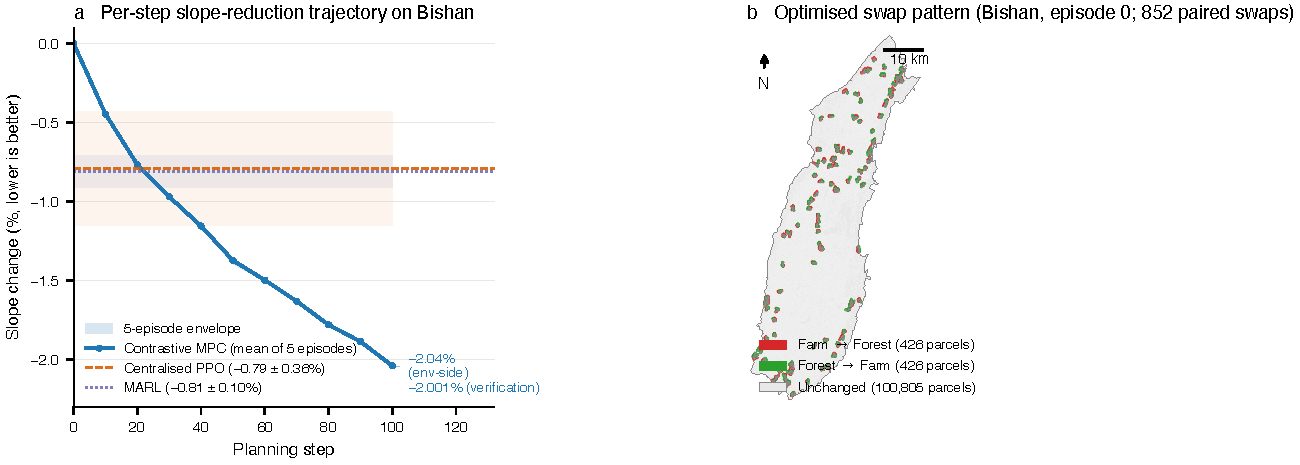
\includegraphics[width=\textwidth]{bishan_headline.pdf}
\caption{Bishan unconstrained candidate scenario and independent audit. (\textbf{a}) Per-step slope-reduction trajectory of the shipped Bishan ensemble on the package-side prepare, mean of five evaluation episodes; the ensemble is deterministic across the action-selection path under fixed seed, so the five episodes overlap to within $0.002$\,pp at every step. Endpoint annotations report the env-side slope ($-2.04\%$) and the independent GIS-only recomputation of $-2.001\%$ (Methods \S\ref{sec:methods-validate}). The dashed line shows the in-house Centralised PPO baseline ($-0.79 \pm 0.36\%$, lab pipeline) and the dotted line shows MARL ($-0.81 \pm 0.10\%$, lab pipeline); the open marker at the corresponding endpoint is the lab-pipeline contrastive-MPC result of $-1.289 \pm 0.079\%$ (5 ensembles $\times$ 1 episode each, Supplementary Table~S9). The DRL baselines were trained on the lab pipeline; the package-side value is not collapsed with the lab-pipeline value because the corrected geographic-CRS slope step exposes truer initial slopes ($9.62^{\circ}$ vs $8.41^{\circ}$). (\textbf{b}) Spatial distribution of the paired swaps committed by the planner on the optimised cadastre (episode~0), shown as farm$\to$forest parcels (red, slope-shed) and forest$\to$farm parcels (green, slope-take), buffered to $250$\,m for visibility at county scale. Swaps concentrate at fragment boundaries where slope-reducing trades cost the least qualifying area. This candidate is useful for audit, but it is not yet a final policy-compliant plan because it reduces total cultivated area by 505\,ha (Supplementary Table~S14).}
\label{fig:bishan-headline}
\end{figure}

The audit explains why candidate generation must be coupled to policy checks. On the package-side prepare, Bishan slope decreases by $2.001\%$, contiguity rises by $0.0128$, and the \textit{baimu fang} count increases by $+8$. The scenario shifts $687$\,ha out of the steep ($\geq 15^\circ$) tail and improves all 13 core townships, but it also reduces qualifying \textit{baimu fang} area by $473$\,ha and total cultivated area by $505$\,ha. We therefore treat it as an informative but rejected candidate: it exposes a high-value slope-contiguity trade-off, while showing that cultivated-area preservation must be a hard execution constraint.

Activating a hard cumulative cultivated-area floor of $0$\,ha converts that audit finding into an executable constraint. The canonical constrained Bishan deployment run reaches $-0.675\%$ slope change, $+0.0204$ contiguity, $+1$ \textit{baimu fang}, $+29.8$\,ha qualifying area and $+3.03$\,ha total cultivated area after $401$ paired swaps, while still shifting $218$\,ha out of the steep tail. Across five independently trained no-net-loss ensembles on the Bishan prepared dataset, slope change is $-0.634 \pm 0.044\%$, contiguity change is $+0.0229 \pm 0.0018$, qualifying \textit{baimu fang} area change is $+22.0 \pm 8.3$\,ha, and cultivated-area change is $+5.39 \pm 5.17$\,ha; all five seeds keep cultivated area non-negative. A seven-profile execution frontier shows the policy trade-off explicitly: no-net-loss profiles retain $-0.608$ to $-0.711\%$ slope change, positive contiguity and $+29.2$ to $+43.4$\,ha qualifying-area gains, whereas looser floors recover more slope gain but remain outside no-net-loss compliance.

For method comparison, we separately use the lab cadastre on which the in-house Centralised PPO and multi-agent baselines were trained. This gives three Bishan numbers with different roles, which we do not average: the package-side GIS anchor ($-2.001\%$) verifies the on-disk candidate geometry; the lab-pipeline value ($-1.289 \pm 0.079\%$) is the matched-cadastre comparison against DRL baselines; and the CLI/toolbox replications test the released workflow (Supplementary Section~S3). The DRL baselines use the same CountyLevelEnv, block-level action space, action mask, reward function and deterministic evaluation protocol as the matched contrastive-MPC comparison; their hyperparameters, seed failures and statistical tests are reported in Supplementary Sections~S1--S3. Across five independently trained contrastive ensembles on the matched lab cadastre, slope change is $-1.289 \pm 0.079\%$, about $1.6\times$ the magnitude of the multi-agent baseline ($-0.81 \pm 0.10\%$; Welch's $p < 10^{-4}$) and Centralised PPO ($-0.79 \pm 0.36\%$; $p = 0.034$), with comparable contiguity and \textit{baimu fang} count. At a matched 180\,s wall budget, simulated annealing reaches reward $9.04$, random restart $30.85$ and contrastive MPC $86.74$; a $10\times$ longer OR budget remains an order of magnitude below contrastive MPC (Supplementary Section~S12). The comparison therefore shows both quality and time asymmetry: contrastive training takes $25$ min on CPU and planning takes about $5$ min per scenario, whereas model-free RL requires $8$--$12$ GPU-hours per seed.

The constrained-repair pattern also appears on Neijiang Dongxing, a larger and more fragmented county ($76{,}376$ parcels, $3{,}711$ blocks). The canonical unconstrained audit again finds a cultivated-area violation ($-261$\,ha), but the corresponding single no-net-loss deployment run repairs it while retaining $-0.492\%$ slope change, $+0.0373$ contiguity, $+252.6$\,ha \textit{baimu fang} area and $+62.2$\,ha cultivated area. GIS-only recomputation of the optimised Neijiang shapefile reproduces these deltas and shows a $330.4$\,ha reduction in farmland within the $\geq 15^\circ$ slope bands. A seven-profile Neijiang execution frontier on the current Scientific Reports prepared package keeps all no-net-loss profiles cultivated-area positive, with $-0.440$ to $-0.457\%$ slope change, $+0.0322$ to $+0.0404$ contiguity and $+286.5$ to $+344.0$\,ha qualifying-area gains. Across five independently trained no-net-loss ensembles on the Neijiang prepared dataset, slope change is $-0.479 \pm 0.042\%$, contiguity change is $+0.0333 \pm 0.0013$, qualifying \textit{baimu fang} area change is $+292.8 \pm 58.2$\,ha, and cultivated-area change is $+107.9 \pm 46.2$\,ha; all five seeds keep cultivated area above the initial value. The \textit{baimu fang} patch count decreases by $11.2 \pm 3.4$, so the constrained evidence supports area-level large-patch improvement but not patch-count improvement. The two-county pattern is therefore consistent, but not a claim of regional generalisation: unconstrained learned planning exposes a useful frontier, and hard execution floors translate that frontier into feasible scenarios.

We also ran retrained reward-weight sensitivity tests in both counties to test whether the constrained outcomes depended on the default \textit{baimu fang} weighting. Each county-profile pair re-ran Tool~2 sampling and Tool~3 ensemble training before no-net-loss Tool~4 planning, so the reward head and the planner used the same profile weights (Methods, \S\ref{sec:methods-reward-sensitivity}). In Bishan, the default, low and high profiles all retained no-net-loss while giving slope changes of $-0.7247\%$, $-0.6522\%$ and $-0.8379\%$, contiguity gains of $+0.0270$, $+0.0209$ and $+0.0343$, and qualifying-area changes of $+27.49$, $+17.34$ and $+56.21$\,ha. In Neijiang, the same profiles retained no-net-loss and reached $-0.4705\%$, $-0.4496\%$ and $-0.4468\%$ slope change, $+0.0278$, $+0.0290$ and $+0.0309$ contiguity, and $+188.60$, $+185.80$ and $+205.63$\,ha qualifying area. Cultivated-area changes remained non-negative in all six runs, ranging from $+0.18$ to $+30.15$\,ha. We use these retrained runs only as a reward-dependence probe. They are not averaged with the canonical deployment runs or the five-ensemble stability sweeps.

\paragraph{Audit boundaries.} We keep three evidence roles separate: the package-side GIS anchors verify on-disk canonical deployment geometry, the lab pipeline supports matched comparison against DRL baselines, and the CLI/toolbox replications test the released workflow (Supplementary Section~S3). Five checks bound the results: independent GIS recomputation reproduces the reported canonical Bishan and Neijiang deployment deltas; 1-step model-audit trajectories show the ensemble is mis-calibrated in reward magnitude but still carries enough ranking signal for the shipped Bishan action path; replacing the ensemble with true \texttt{env.step} under matched concessions performs worse than the batched ensemble planner; five-ensemble no-net-loss sweeps in Bishan and Neijiang estimate training-seed stability of the cultivated-area floor; and reward-weight sensitivity in both counties re-runs sampling and training under lower/default/higher \textit{baimu fang} weights. These variance and sensitivity sweeps are computed inside the prepared CountyLevelEnv and do not replace the canonical GIS-only recomputation.

% ============================================================================
\subsection{Cross-landscape stress test on a synthetic benchmark}\label{sec:bench}
% ============================================================================

To test whether the result depends on properties shared by Bishan and Neijiang (both situated in southwestern hilly terrain), we constructed a synthetic benchmark of seven parametric landscapes varying along three morphological axes: terrain (hilly, mixed, plain), problem size ($800$, $2{,}600$, $4{,}500$ blocks), and fragmentation (consolidated, fragmented). Two presets are calibrated against the real anchors; the remaining five are parameter-controlled stress tests (Methods, \S\ref{sec:methods-synth}). All seven landscapes plus the deterministic generator are released under CC-BY 4.0 (\S Data Availability), so external researchers can reproduce the open benchmark experiments and test future methods without access to restricted cadastral records.

We benchmarked five methods (uniform-random selector, slope-greedy heuristic, genetic algorithm \citep{cao2012boundary}, centralised PPO, contrastive MPC) on the seven landscapes with five random seeds each (full slope-improvement profile in Supplementary Table~S5). Two patterns mark the boundary of the claim. On the five presets that are large or fragmented enough to make multi-step planning informative (the two real-data clones plus three medium--large fragmented presets), contrastive MPC is the strongest method, with PPO the consistent runner-up; the MPC slope-improvement margin over the genetic algorithm is $6$--$54\%$ across these cells, and remains $37\%$ even on the largest preset ($4{,}500$ blocks, $\sim$$9.3$\,h MPC wall time vs $\sim$$248$\,s GA). On the small consolidated preset (\texttt{plain\_small\_cons}, $800$ blocks), the genetic algorithm wins ($-2.757 \pm 0.203\%$ vs.\ MPC $-2.226 \pm 0.220\%$): the action space is small enough that GA's population-based exploration covers it within budget, and the planning value of contrastive ranking, which scales with the within-state action menu, is muted. These synthetic landscapes are stress tests rather than representative counties. They support the regime structure read from \S\ref{sec:counties}--\S\ref{sec:cross-domain}: contrastive MPC is the strong method when the problem is large or fragmented enough to make per-state ranking matter; classical search wins when it is not.

% ============================================================================
\subsection{Cross-domain boundary check on a public-data restoration case}\label{sec:cross-domain}
% ============================================================================

To bound the contrastive intervention, we apply the unmodified pipeline to ecological-restoration prioritisation for abandoned mine lands. The real case is Buchanan County, Virginia ($562$ public-data planning cells from OSMRE e-AMLIS, USGS NHD, USGS 3DEP and Census TIGER); the second is a deterministic synthetic case with $420$ units. In both, reward is a per-unit attribute lookup combining risk reduction, water-quality protection, spatial connectivity and cost (Methods, \S\ref{sec:methods-restoration}).

Across seven methods (Table~\ref{tab:restoration-baselines}), the contrastive loss provides no operational advantage over MSE-only learned MPC: on Buchanan the two agree within $0.20$ reward units, pairwise ranking accuracy is $\geq 0.95$ for both, and top-$K$ regret is $<0.003$ at $K{=}1$. This matches the diagnostic from \S\ref{sec:rank}: restoration has large within-state action variance ($\sigma_a/\sigma_s \approx 5$--$7$), so MSE training already learns the ranking signal. Classical OR baselines also reach near-optimum, unlike farmland where simulated annealing reaches reward $9.04$ versus contrastive MPC's $86.74$ at matched wall budget. The toggling factor is simulator cost, developed next.

\begin{table}[htbp]
\centering
\small
\caption{Optimisation results across seven methods on the two restoration cases (cumulative episode reward; mean $\pm$ std for stochastic methods, $n=5$ seeds where applicable; deterministic methods are single runs). The greedy heuristic, simulated annealing, and CBC-MILP weighted-sum baselines reach near-optimum on both cases, statistically indistinguishable from the learned-surrogate MPC variants. The advantage of the learned-surrogate pipeline over the OR baselines is therefore not the optimum quality on this case; it is the wall-clock and the ability to absorb new reward-weight configurations without re-running the optimiser (\S\ref{sec:methods-restoration}).}
\label{tab:restoration-baselines}
\resizebox{\textwidth}{!}{%
\begin{tabular}{lccc@{\hspace{1em}}ccc}
\toprule
 & \multicolumn{3}{c}{Buchanan VA (real, $n=562$)} & \multicolumn{3}{c}{Synthetic (deterministic, $n=420$)} \\
\cmidrule(lr){2-4}\cmidrule(lr){5-7}
Method & total reward & $n_{\text{sel}}$ & wall-time (s) & total reward & $n_{\text{sel}}$ & wall-time (s) \\
\midrule
random (uniform) & $+88.7 \pm 12.7$ & 50.0 & $<0.1$ & $+6{,}163 \pm 160$ & 59.8 & $<0.1$ \\
greedy by priority & $+228.76$ & 50 & $<0.1$ & $+8{,}590.9$ & 60 & $<0.1$ \\
simulated annealing & $+228.76$ & 50 & 0.7 & $+8{,}737.0$ & 60 & 0.6 \\
NSGA-II (4-obj) & $+175.45$ & 50 & 3.2 & $+7{,}075.7$ & 60 & 2.9 \\
CBC-MILP weighted-sum & $+229.43$ & 50 & 3.0 & $+8{,}127.2$ & 49 & $<0.1$ \\
MSE-only MPC ($\lambda{=}0$) & $+229.20 \pm 0.14$ & 50 & $\sim 28$ & $+8{,}173 \pm 66$ & 60 & $\sim 5$ \\
\textbf{contrastive MPC ($\lambda{=}5$)} & $\mathbf{+229.39 \pm 0.03}$ & 50 & $\sim 28$ & $\mathbf{+8{,}128 \pm 63}$ & 60 & $\sim 5$ \\
\bottomrule
\end{tabular}
}
\end{table}


\begin{figure}[htbp]
\centering
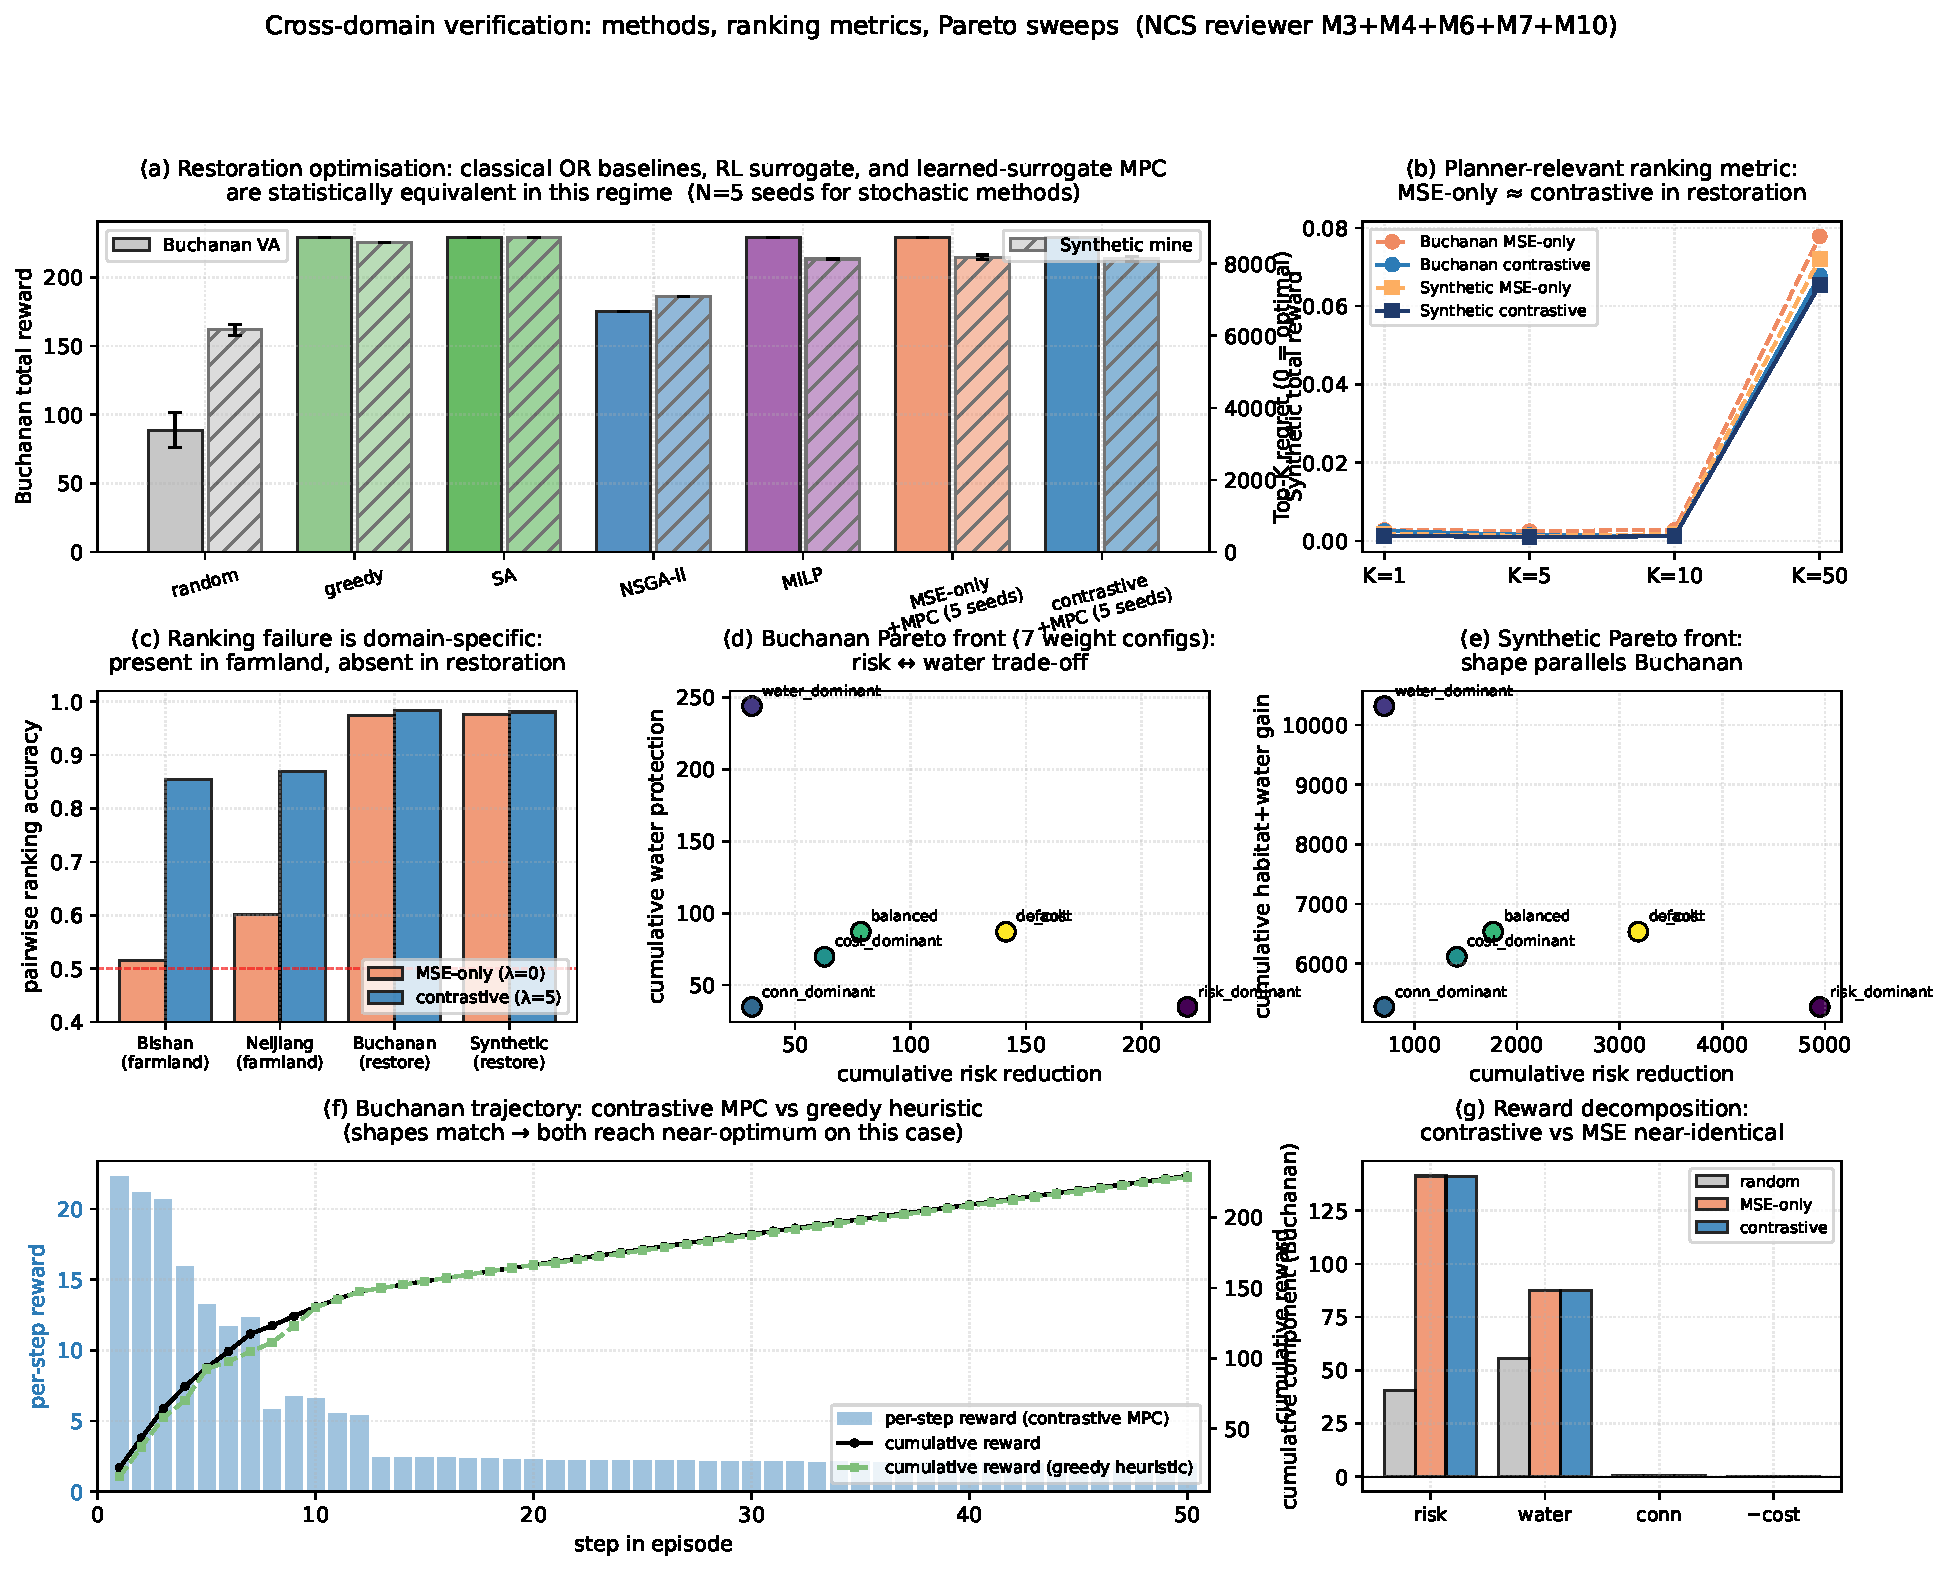
\includegraphics[width=\textwidth]{figure_restoration.pdf}
\caption{Cross-domain boundary check, expanded baseline panel, and Pareto front. (a)~Cumulative episode reward across seven methods on Buchanan (left axis) and synthetic (right axis); MSE-only and contrastive learned-MPC variants are statistically indistinguishable from greedy-by-priority and CBC-MILP, all far above the random baseline. (b)~Top-$K$ regret as a function of $K$: MSE-only and contrastive surrogates are equivalent on both cases, indicating that the contrastive intervention has little headroom in the restoration regime. (c)~Pairwise ranking accuracy across all four domains: farmland (Bishan, Neijiang) shows the large MSE-vs-contrastive gap, restoration (Buchanan, synthetic) shows MSE-only already saturating. (d, e)~Pareto front of cumulative risk reduction vs cumulative water/habitat protection across seven reward-weight configurations on Buchanan and synthetic respectively; the shape is consistent across cases. (f)~Trajectory comparison on Buchanan: per-step reward (bars) and cumulative reward (line) for contrastive MPC vs the greedy heuristic; both reach the same end state via similar action sequences, showing that the OR baseline is a strong reference on this case. (g)~Reward-component decomposition: contrastive vs MSE-only allocate cumulative reward across the four objective terms within noise.}
\label{fig:restoration-pareto}
\end{figure}

% Synthesis paragraph removed for length; the regime-conditional framing is
% folded into Discussion and into §sec:simcost which immediately follows.

% Pareto-aware figures and the original boundary-check figure:
% restoration_verification_v2 (figure above) supersedes the older restoration figure
% which is retained for compatibility but no longer referenced in the main text.

% ============================================================================
\subsection{Simulator step cost as an empirical diagnostic for MPC-vs-OR advantage}\label{sec:simcost}
% ============================================================================

To evaluate whether simulator cost explains the farmland/restoration split, we inject fixed delays of \{0, 1, 10, 50, 100\}\,ms into each restoration \texttt{env.step} and re-run simulated annealing and learned MPC at matched 30-second budgets across ten (case~$\times$~reward-profile) cells (Methods, \S\ref{sec:methods-simcost}).

\begin{figure}[htbp]
\centering
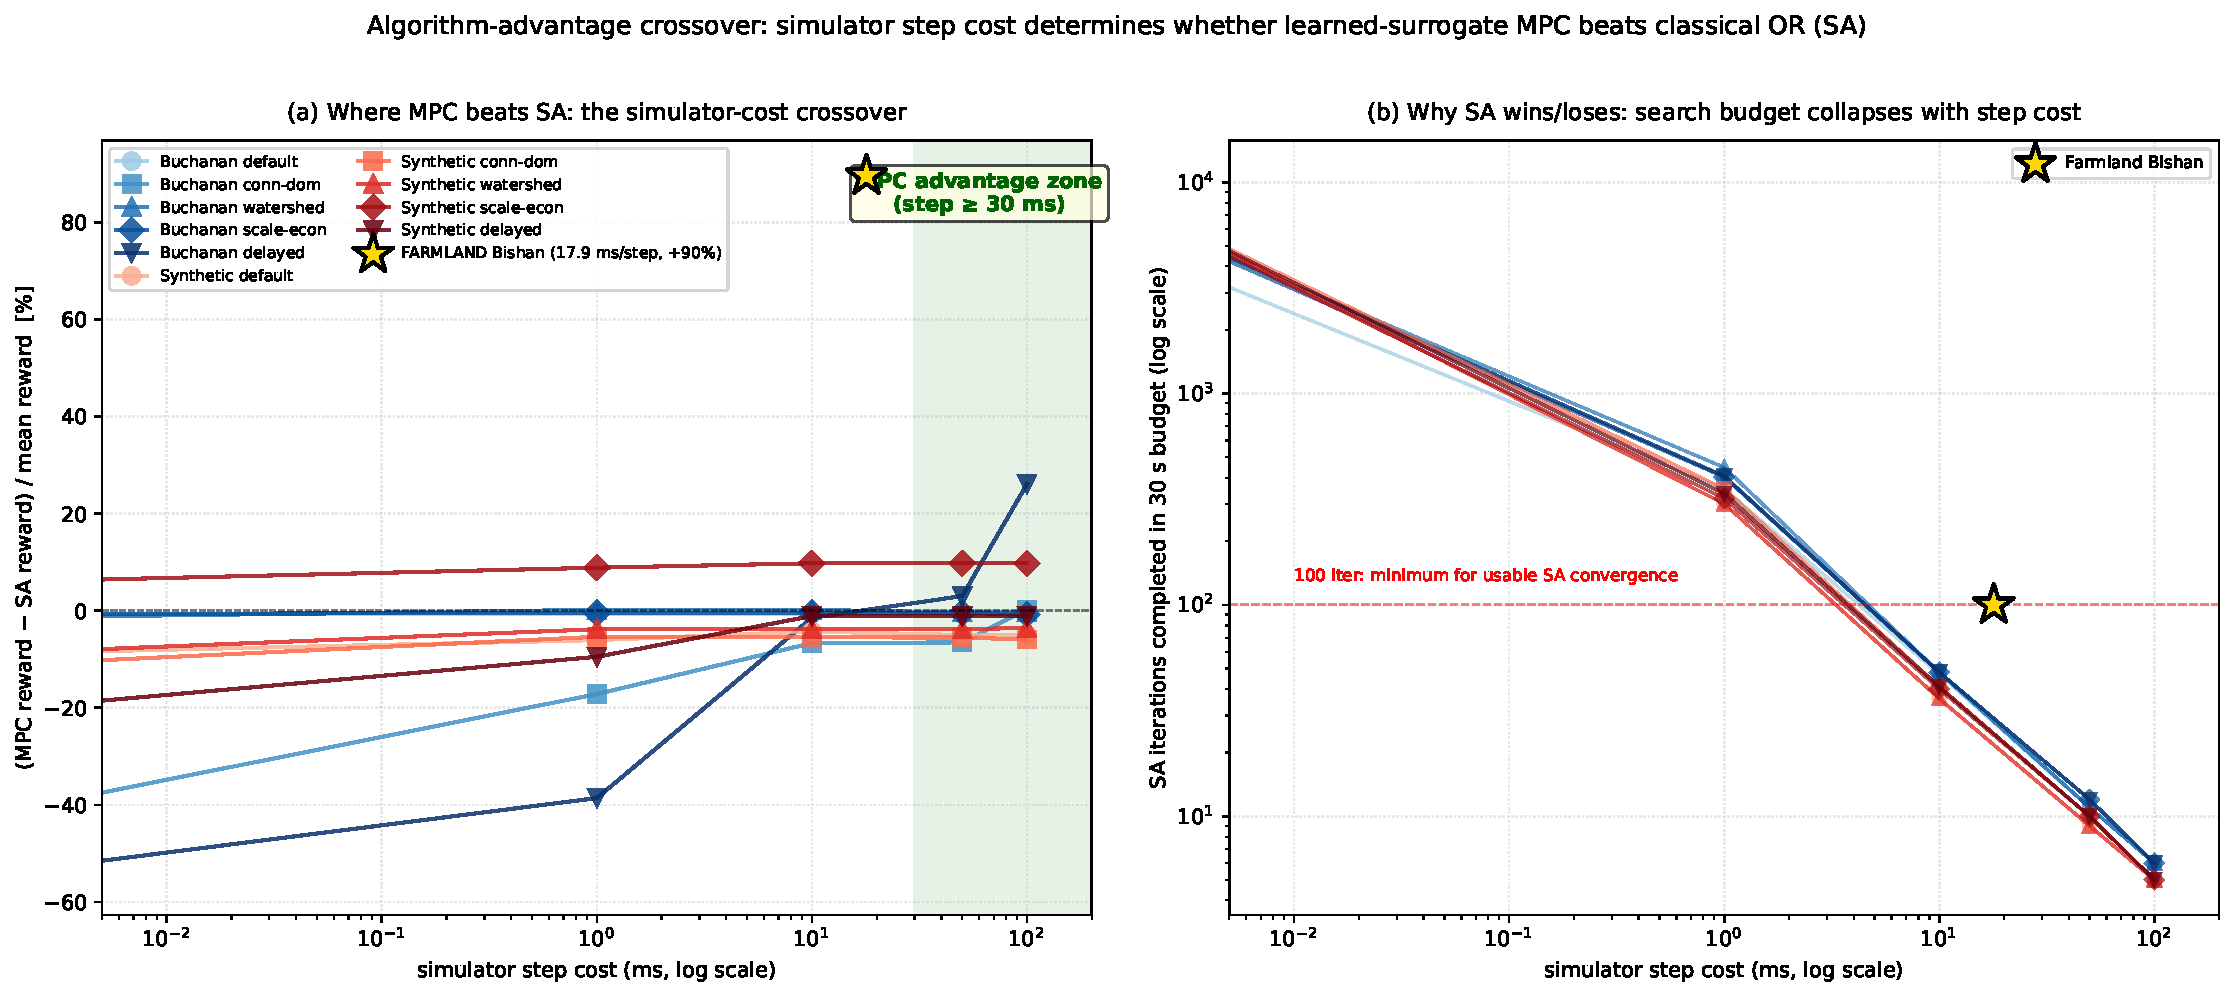
\includegraphics[width=\textwidth]{figure_simcost.pdf}
\caption{Simulator step cost is an empirical diagnostic for when learned-surrogate MPC beats simulated annealing under matched wall-clock budgets. (a)~Reward gap (MPC minus SA, normalised by per-cell mean reward) versus injected step delay (log scale) on ten (case~$\times$~reward-profile) cells. The shaded green band marks the empirical MPC-advantage zone observed on these ten cells (transition near $30$\,ms/step); we report this as an empirical inflection rather than a universal threshold. The actual farmland Bishan datapoint (gold star), measured at $17.9$\,ms/step natural step cost under a 180\,s wall budget, sits at $+89.6\%$. (b)~SA iteration count completed in the same wall budget on a log-y axis: the count collapses linearly with step cost from $\sim 9{,}000$ at 5\,$\mu$s/step to $\sim 6$ at 100\,ms/step. Below $\sim 100$ iterations SA cannot converge, the mechanism by which step cost translates into the MPC advantage. The synthetic/scale\_economy line is the exception: MPC dominates at every step delay because its combinatorial cost-interaction structure is what learned-surrogate batched scoring exposes naturally.}
\label{fig:simcost}
\end{figure}

On nine of ten attribute-lookup cells, the MPC-vs-SA gap is monotonic in delay: SA completes $\sim 9{,}000$ iterations at near-zero delay but only $\sim 6$ at 100\,ms, while learned MPC pays one $\sim 25$\,ms batched ONNX call over $K{=}50$ candidates. The crossover occurs near $30$\,ms/step on the tested cells. The remaining synthetic/scale-economy cell shows a second factor, combinatorial cost interactions, where MPC dominates even at near-zero delay because the learned surrogate scores actions in the current joint state. Farmland combines both factors: Bishan's natural step cost is $17.9 \pm 0.3$\,ms and its reward aggregates slope, contiguity and \textit{baimu fang} connectivity after every swap. We therefore propose two problem-selection diagnostics, simulator step cost and combinatorial reward structure, while treating the $30$\,ms value as empirical rather than universal.

% ============================================================================
\subsection{From paper to planner's desk: an end-to-end deployment toolchain}\label{sec:deploy}
% ============================================================================

For deployment, we package the pipeline as an ArcGIS Pro Python Toolbox plus a QGIS-compatible command-line workflow. The four tools prepare cadastral blocks from a DLTB shapefile and DEM, sample the pairwise dataset, train the contrastive ensemble and write an optimised cadastral shapefile; a fifth diagnostic tool checks dependencies before execution (Figure~\ref{fig:toolchain}).

\begin{figure}[htbp]
\centering
\resizebox{\textwidth}{!}{%
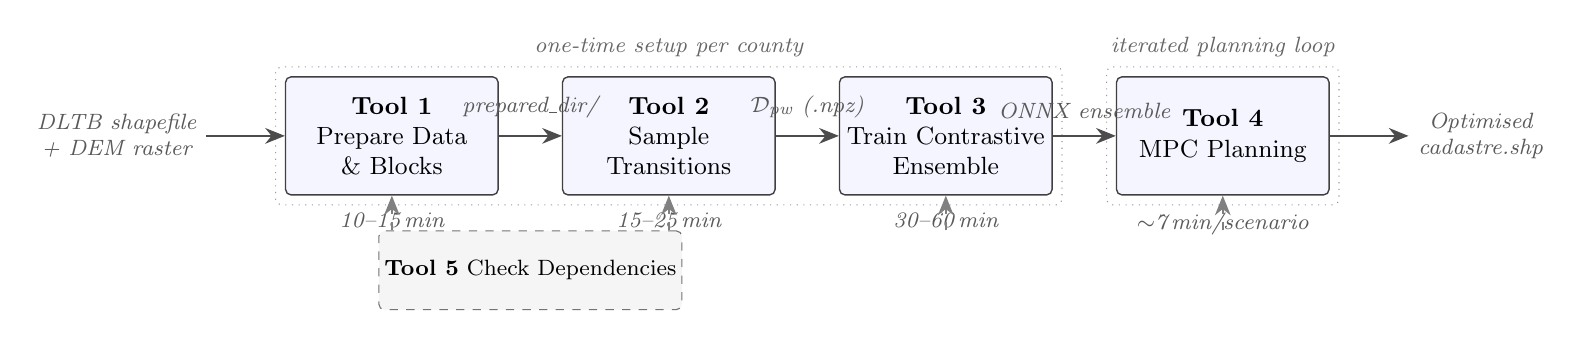
\begin{tikzpicture}[
  font=\small,
  node distance=6mm and 8mm,
  tool/.style={rectangle, rounded corners=2pt, draw=black!75, line width=0.5pt,
               minimum width=27mm, minimum height=15mm, align=center,
               fill=blue!4, inner sep=2pt},
  io/.style={font=\footnotesize\itshape, text=black!65, align=center},
  flow/.style={-{Stealth[length=2.5mm,width=2mm]}, line width=0.6pt, draw=black!70},
  check/.style={rectangle, rounded corners=2pt, draw=black!55, dashed, line width=0.4pt,
                minimum width=27mm, minimum height=10mm, align=center,
                fill=gray!8, inner sep=2pt, font=\footnotesize}
]
% Inputs
\node[io] (in) {DLTB shapefile\\+ DEM raster};

% Four tools left to right
\node[tool, right=10mm of in]              (t1) {\textbf{Tool 1}\\Prepare Data\\\& Blocks};
\node[tool, right=of t1]                   (t2) {\textbf{Tool 2}\\Sample\\Transitions};
\node[tool, right=of t2]                   (t3) {\textbf{Tool 3}\\Train Contrastive\\Ensemble};
\node[tool, right=of t3]                   (t4) {\textbf{Tool 4}\\MPC Planning};

% Output
\node[io, right=10mm of t4] (out) {Optimised\\cadastre.shp};

% Inter-tool I/O hints (above each arrow)
\node[io, above=1mm of $(t1)!0.5!(t2)$] {prepared\_dir/};
\node[io, above=1mm of $(t2)!0.5!(t3)$] {$\mathcal{D}_{\text{pw}}$ (.npz)};
\node[io, above=1mm of $(t3)!0.5!(t4)$] {ONNX ensemble};

% Wall-time hints (below)
\node[io, below=1mm of t1] {10--15\,min};
\node[io, below=1mm of t2] {15--25\,min};
\node[io, below=1mm of t3] {30--60\,min};
\node[io, below=1mm of t4] {$\sim$7\,min/scenario};

% Flow arrows
\draw[flow] (in)--(t1);
\draw[flow] (t1)--(t2);
\draw[flow] (t2)--(t3);
\draw[flow] (t3)--(t4);
\draw[flow] (t4)--(out);

% One-time vs iterated bracket
\begin{scope}[on background layer]
\node[draw=black!40, dotted, rounded corners=2pt, line width=0.4pt,
      fit=(t1)(t2)(t3),
      label={[font=\footnotesize\itshape, text=black!60]above:one-time setup per county}] (setup) {};
\node[draw=black!40, dotted, rounded corners=2pt, line width=0.4pt,
      fit=(t4),
      label={[font=\footnotesize\itshape, text=black!60]above:iterated planning loop}] (plan) {};
\end{scope}

% Tool 5 sidecheck
\node[check, below=12mm of $(t1)!0.5!(t2)$] (t5) {\textbf{Tool 5} Check Dependencies};
\draw[flow, dashed, draw=black!50] (t5.north -| t1.south) -- (t1.south);
\draw[flow, dashed, draw=black!50] (t5.north -| t2.south) -- (t2.south);
\draw[flow, dashed, draw=black!50] (t5.north -| t3.south) -- (t3.south);
\draw[flow, dashed, draw=black!50] (t5.north -| t4.south) -- (t4.south);

\end{tikzpicture}%
}
\caption{The four-tool ArcGIS Pro deployment pipeline (\S\ref{sec:methods-toolchain}). Tools~1--3 run once per county to prepare cadastral data, sample the pairwise dataset, and train the contrastive transition-model ensemble (exported to ONNX). Tool~4 is the iterated planning loop a county officer runs repeatedly under different reward weightings; one 100-step scenario finishes in $\sim$7\,min on a desktop CPU. A separate Tool~5 (dashed) validates the Python environment, Spatial Analyst availability, and ONNX shape compatibility before any pipeline run is allowed.}
\label{fig:toolchain}
\end{figure}

Tools 1--3 take $\sim$1--2\,h once per county; Tool 4 runs a scenario in $\sim$7\,min. A full UI-driven Bishan run yields $-1.544 \pm 0.041\%$ slope change across five episodes, consistent in direction and scale with the lab comparison. The MIT-licensed package, CC-BY synthetic benchmark, trained ensembles, Buchanan restoration case and smoke test form the open reproduction kit, while restricted raw cadastral records remain governed as described in Data availability.

% ============================================================================
\section{Discussion}\label{sec:discussion}
% ============================================================================

\paragraph{What the pipeline delivers for sustainability planning.} The operational shift is from slow optimisation runs to fast, auditable scenario generation. In Bishan and Neijiang, unconstrained high-slope candidates are useful because they expose the slope-retirement frontier, but both lose cultivated area and should be rejected as final plans. Hard cultivated-area floors convert that audit into an execution constraint while preserving positive slope, contiguity and large-patch gains. The percentage slope changes are modest because they are county-wide area-weighted means; in the audited constrained runs they correspond to $218$\,ha (Bishan) and $330$\,ha (Neijiang) less farmland in the $\geq 15^\circ$ slope bands. These constrained scenarios are decision-support artefacts. The present state representation does not encode parcel ownership, soil quality, irrigation access, ecological red lines, construction or transaction costs, or stakeholder consent. The outputs therefore still require local review of land tenure, ecology and administrative feasibility. The practical value is not autonomous plan approval, but a faster loop between candidate generation, GIS verification and policy thresholds.

\paragraph{Mechanism and transfer.} Two diagnostics explain when the approach helps in our experiments. The pairwise ranking loss closes an MSE ranking failure when $\sigma_a/\sigma_s \!\lesssim\! 1$, but is redundant when reward is a per-unit attribute lookup. The learned-surrogate planner beats classical OR when simulator steps are costly or rewards contain combinatorial interactions, with a tested crossover near $30$\,ms/step on the restoration cells rather than a universal threshold. Supplementary H/K sweeps show that one released Bishan ensemble is invariant to planning depth and candidate width over the tested grid, and extended-wall-budget OR runs remain below contrastive MPC on Bishan. These are problem-selection diagnostics, not a general theory of surrogate planning. Practitioners should therefore report simulator step cost, reward structure, constraint status and planning-budget sensitivity before adopting the method.

\paragraph{Bounds on the claim.} The evidence is bounded by two real counties in southwestern China, restricted raw cadastral records, a pairwise dataset that relies on simulator snapshot/restore, and diagnostics calibrated on farmland plus restoration rather than on physics-driven Earth-science simulators. The reward weights are inherited from the in-house baseline configuration and are held fixed for the main method comparisons; they should be read as transparent objective coefficients, not as calibrated social-welfare or statutory preference weights. The added reward-weight sensitivity shows that no-net-loss planning remains feasible in both counties under halved and doubled \textit{baimu fang} terms, and that the higher-weight profile increases qualifying-area response in both counties. It is therefore evidence against a trivial default-weight artefact. It is still not a full Pareto analysis because each county-profile cell uses one retrained three-member ensemble and one deterministic planning episode. The five-ensemble no-net-loss sweeps and two county-level execution frontiers address whether the cultivated-area floor remains feasible across independently trained ensembles and across policy-floor settings in the two counties tested; they do not replace broader constrained-frontier evidence across additional counties. The no-net-loss cultivated-area floor is a necessary deployment constraint in this study, but it is not a complete substitute for statutory review or local plan approval. The immediate follow-up is therefore a broader constrained-frontier study with retrained reward weights across additional counties and policy floors.

% ============================================================================
\section{Methods}
\label{sec:methods}
% ============================================================================

\paragraph{Scope and architectural framing.} The architecture used throughout this paper is a feed-forward deterministic learned transition model with a discriminative reward head (\S\ref{sec:methods-action} below). It is in the operational sense of \citet{chua2018deep} and \citet{janner2019trust} a learned $\hat{p}(s_{t+1}, r_t \mid s_t, a_t)$ that substitutes for the real environment in MPC lookahead and simulated policy training. The task is fully observed (state is the per-block 17-dim feature vector emitted by Tool 1; no raw observation), episodic (100-step cap, no partial observability), and the action space is finite categorical of size $N_{\text{blocks}}$ (Methods, \S\ref{sec:methods-action}). We therefore do not learn a representation from raw observations, do not use recurrent latent dynamics, and do not claim a general-purpose world-model architecture. The reported contribution is instead the ranking diagnostic, the constrained audit and the deployable GIS workflow.

\subsection{Per-parcel slope from DEM and cadastral polygons}\label{sec:methods-prepare}

The per-parcel slope feature used throughout the analysis is derived from the Third National Land Survey cadastral polygons and Copernicus DEM GLO-30 elevation tiles \citep{copernicus2021dem}, both freely available in their respective public archives. The DEM is kept in its native geographic CRS (EPSG:4326, 1-arcsecond resolution); slope is computed by central-difference gradients on the elevation grid using true east-west and north-south metres-per-pixel obtained from \texttt{pyproj.Geod} (WGS84 ellipsoid) at the study-area centre latitude. The pixel spacing is $\sim$$27$\,m east-west and $\sim$$31$\,m north-south at $29.5^\circ$N (the centre of both Bishan and Neijiang); reprojecting the DEM to a metric projection before gradient differencing would average over these non-square cells and systematically under-estimate slope. The slope raster, in degrees, is then aggregated to each cadastral polygon by area-weighted zonal mean over all DEM cells whose centre falls within the polygon. Polygons that contain no cell centre (typically very small parcels, $\lesssim 30$\,m linear scale) inherit the per-county median slope to keep the downstream feature vector finite; on Bishan and Neijiang this affects $\sim$$2$\% and $\sim$$3$\% of parcels respectively, all in the smallest size class. The full prepare pipeline (DEM merge $\to$ slope $\to$ zonal mean $\to$ per-township block construction) takes $\sim$$3$ minutes on Bishan and $\sim$$5$ minutes on Neijiang on a 14-core desktop CPU and is released as the \texttt{farmland-mpc prepare} command (\S Code Availability).

\subsection{Problem setting and action-space encapsulation}\label{sec:methods-action}

We study county-level farmland consolidation in two real counties (Bishan District, Chongqing; Neijiang Dongxing District, Sichuan) and seven synthetic landscapes (\S\ref{sec:methods-synth}). For Bishan, the planning area comprises 13 townships, $2{,}600$ spatial blocks, and $52{,}515$ cadastral parcels; for Neijiang, 29 townships, $3{,}711$ blocks, and $76{,}376$ parcels (Supplementary Table~S1). Each block aggregates multiple parcels and is characterised by 17 features (farmland area, forest area, slope statistics, adjacency metrics, and investment indicators). Global context is encoded as an additional 12 features (remaining budget, contiguity, \textit{baimu fang} count, etc.). The episode length is fixed at 100 steps for the real-data experiments and 50 steps for the synthetic benchmark (\S\ref{sec:bench}); each step has a budget of up to 5 paired farmland--forest swaps.

\paragraph{Agent action space.}
The agent's action space is a single categorical choice over the spatial blocks per step: $a_t \in \{1, \ldots, N_{\text{blocks}}\}$. The agent does \emph{not} select individual parcels or the paired-swap sub-actions. Given the selected block, the environment internally executes \emph{up to} 5 paired farmland--forest swaps within that block using a deterministic rule-based procedure: candidate pairs are enumerated by joint feasibility under farmland--forest pairing and slope constraints, scored by a local improvement heuristic, and the top-scoring feasible pairs are applied until either 5 pairs are executed or the candidate pool is exhausted. The agent therefore chooses \emph{where} to act, not \emph{what} to do within the chosen location; this encapsulation keeps the action space at a tractable scale ($\sim 10^3$). The paired farm$\leftrightarrow$forest swap conserves \emph{counts} (one farmland parcel out, one forest parcel in) but not \emph{areas}: parcels are paired by class and by within-block proximity, not by area, so any net cultivated-area change across an episode reflects the planner's slope reward favouring high-slope (typically large) farmland exit and low-slope (typically small) forest entry. The unconstrained Bishan candidate scenario described in \S\ref{sec:counties} loses $505$\,ha ($1.05\%$) of total cultivated area as a consequence. This is not a hidden implementation detail; it is a failed hard constraint surfaced by the independent audit. The constrained runs reported in \S\ref{sec:counties} activate \texttt{cultivated\_area\_floor\_delta\_ha}; with the default value $0.0$, each committed pair must keep cumulative cultivated area at or above its initial value. A second execution floor, \texttt{baimu\_area\_floor\_delta\_ha}, can reject pairs that would push cumulative qualifying \textit{baimu fang} area below a user-specified threshold. The connectivity-conservative profile reported in Supplementary Table~S17 uses the same action path but increases local pair-selection weights \texttt{gamma\_conn} and \texttt{delta\_conn} to favour swaps that preserve farmland adjacency during execution.

\paragraph{Action masking.}
Not all blocks are legal targets at every step. The action mask $m_t \in \{0, 1\}^{N_{\text{blocks}}}$ disables blocks that (i) have no remaining feasible parcel pairs under the local farm--forest and slope rules, (ii) are currently in a township whose per-township swap budget has been exhausted, or (iii) have been selected in the immediately previous step (a simple debounce to prevent action thrashing). MaskablePPO \citep{ross2011reduction,schulman2017proximal,huang2022maskable}-style masking is applied in both the policy sampling and the MPC candidate enumeration, so that illegal blocks have zero probability or are excluded from the $K$ candidate set. When the cultivated-area floor is active, the same mask additionally excludes any block for which no slope-improving within-block pair can be committed without violating the cumulative area floor; the greedy execution loop applies the same test again before every parcel-pair swap. The \textit{baimu fang}-area floor is evaluated in the execution loop rather than in the full action mask because it requires a connected-component recomputation after tentative parcel-pair changes; if no candidate pair in a selected block can satisfy the floor, that block is removed from further execution in the current episode.

\subsection{Reward formulation}\label{sec:methods-reward}

Each step's reward combines three normalised directional signals (slope, contiguity, and qualifying-patch area), a large-patch formation bonus, and an asymmetric area-protection penalty. Let $\bar{\sigma}_t$ be the area-weighted mean farmland slope at step $t$, $C_t$ the within-farmland contiguity index, $B_t$ the count of qualifying \textit{baimu fang} ($\geq$6.67\,ha contiguous farmland patches), and $A_t$ their total area. The per-step reward is
\begin{equation}
\label{eq:reward}
r_t \;=\; w_S \cdot \Delta \bar{\sigma}_t
       \;+\; w_C \cdot \Delta C_t
       \;+\; w_A \cdot \Delta A_t
       \;+\; b_B \cdot \max(0,\, B_t - B_{t-1})
       \;+\; p_A \cdot \min(0,\, \Delta A_t)
\end{equation}
where the directional changes are normalised by their initial county-wide values: $\Delta \bar{\sigma}_t = (\bar{\sigma}_{t-1} - \bar{\sigma}_t)/\bar{\sigma}_0$ (so that slope \emph{reduction} contributes positively), $\Delta C_t = (C_t - C_{t-1})/C_0$, and $\Delta A_t = (A_t - A_{t-1})/A_0^{\mathrm{farm}}$ (normalised by the initial total farmland area $A_0^{\mathrm{farm}}$, so the weights act on relative rather than absolute changes). Weights $(w_S, w_C, w_A, b_B, p_A) = (4000, 500, 1500, 5, 2000)$ are inherited from our in-house DRL baseline configuration and are objective coefficients for matched algorithm comparison, not calibrated welfare, cost-benefit or statutory preference weights. The fourth term is a one-off bonus applied each time the qualifying-patch count increases between steps; the fifth term, $p_A \cdot \min(0, \Delta A_t)$, is an asymmetric penalty that activates only when qualifying area decreases, roughly doubling the marginal cost of shedding \textit{baimu fang} area relative to the symmetric $w_A$ reward (this asymmetry is what drives the agent to consolidate many small qualifying patches into fewer larger ones, increasing total qualifying \emph{area} even as the qualifying \emph{count} falls; \S\ref{sec:counties}). Under a median single-step decomposition, slope improvement contributes $\sim$60\%, contiguity $\sim$15\%, qualifying-patch area $\sim$20\%, and the formation bonus $\sim$5\%. We did not re-tune the weights for the present experiments; contrastive MPC, policy training in the learned-model environment, and the model-free baselines all use the identical reward function, so any method-wise difference is attributable to the learning procedure rather than to reward engineering. A separate fixed penalty of $-1$ is applied whenever a selected block admits no feasible paired swap, discouraging wasted actions. Throughout the paper, ``Slope \%'' is the relative change $\text{Slope \%} = (\bar{\sigma}_T - \bar{\sigma}_0)/\bar{\sigma}_0 \times 100$; contiguity and \textit{baimu fang} count/area changes are absolute.

\paragraph{Retrained reward-weight sensitivity.}\label{sec:methods-reward-sensitivity}
For the reward-weight sensitivity in \S\ref{sec:counties}, we did not change reward weights only at Tool~4 planning time, because the ONNX reward head would then still rank actions under the weights used during Tool~2 sampling and Tool~3 training. Instead, each Bishan and Neijiang profile copied its county-specific prepared template, re-ran Tool~2 with the profile weights, re-trained a three-member contrastive ensemble, and then ran Tool~4 with the hard cultivated-area floor \texttt{cultivated\_area\_floor\_delta\_ha=0}. The default profile used $(w_S,w_C,w_A,b_B,p_A)=(4000,500,1500,5,2000)$; the low profile used $(4000,500,750,2.5,1000)$; and the high profile used $(4000,500,3000,10,4000)$. Each county-profile run used $60$ random-policy transition episodes, $1{,}000$ pairwise states, $50$ actions per state, three ensemble members, up to $30$ epochs with patience $8$, $H{=}5$, $K{=}50$, $\gamma{=}0.99$, greedy continuation, reward scoring and seed $0$. The internal ONNX inference batch size for the final planning rerun was $256$; this is a memory-management parameter only and does not alter the candidate set, objective, horizon or execution floor.

\subsection{Block-level transition model}

The transition model is a feed-forward neural network with approximately $237{,}000$ parameters that takes as input the current block features (all blocks, 17 dimensions each), the global features (12 dimensions), and the selected action (block index), and predicts the next-step block features, global features, and scalar reward. Only the selected block changes (residual formulation). The base loss is
\begin{equation}
\mathcal{L}_{\text{MSE}} = \mathrm{MSE}(\Delta\hat{b}, \Delta b) + \mathrm{MSE}(\Delta\hat{g}, \Delta g) + 0.1 \cdot \mathrm{MSE}(\hat{r}, r),
\end{equation}
trained with Adam (learning rate $10^{-3}$, weight decay $10^{-5}$) on a 90/10 train/validation split with patience-6 early stopping.

\subsection{Ensemble uncertainty estimation}

We train 3--5 independently initialised transition models on the same dataset with different random seeds \citep{lakshminarayanan2017simple}. At inference, the ensemble produces mean predictions for next state and reward, plus the reward standard deviation $\sigma_r$ across members. The simulated learned-model environment penalises high-disagreement actions: $r_{\text{out}} = \bar{r} - \lambda_{\text{disag}} \cdot \sigma_r$ with $\lambda_{\text{disag}} = 0.5$.

\subsection{Policy architecture: parcel-scoring policy}

The policy is a dimension-invariant scoring network compatible with MaskablePPO. For each block $i$, the scorer concatenates the block's 17-dimensional local features with the 12-dimensional global state, passes the result through a shared MLP ($[64, 32] \to 1$), and produces a scalar score. The action is the highest-scoring valid block. A separate value network takes only the global features and predicts the state value.

\subsection{Dataset-aggregation iterative refinement}

We adopt a dataset-aggregation loop following the logic of DAgger \citep{ross2011reduction}: (1)~collect an initial dataset $D_0$ of $6{,}000$ transitions from random and greedy policies on the real environment; (2)~train the transition model ensemble on $D_{\leq i}$; (3)~train a policy in the simulated learned-model environment for $50{,}000$ timesteps; (4)~evaluate on the real environment; (5)~collect 10 stochastic on-policy episodes ($\sim$$1{,}000$ transitions) and augment the dataset. Three iterations are performed.

\subsection{Targeted evidence collection and stabilisation}

In targeted evidence collection, step (5) above is modified: each transition is scored by ensemble reward disagreement $\sigma_r$, and only transitions exceeding threshold $\tau = 0.5$ are retained; under this threshold, $\sim$$99.6\%$ of transitions are filtered out, accounting for the simulated-policy slowdown documented in \S\ref{sec:rank}. Three stabilisation mechanisms are applied across all protected runs. \emph{Best-checkpoint selection}: every $10{,}000$ PPO timesteps, the current policy is evaluated on the real environment (3 episodes); the checkpoint with the highest mean reward is retained. \emph{Iteration-1 rollback}: if iteration-1 reward drops more than 50 points below iteration-0, the dataset and policy are reverted. \emph{Early stopping}: training halts if validation loss does not improve for 6 consecutive epochs.

\subsection{Model-predictive planning protocol}\label{sec:methods-mpc}

We use random shooting model-predictive control \citep{garcia1989model,williams2017model,rubinstein1999cross}. At each real-environment step $t$ with state $s_t$:
\begin{enumerate}
\item Sample $K$ random action sequences $\{a^{(k)}_{t:t+H-1}\}_{k=1}^K$, each of length $H$, from the action-masked support.
\item For each sequence, roll forward through the ensemble mean model: $\hat{s}^{(k)}_{t+1}, \hat{r}^{(k)}_t = f_\theta(s_t, a^{(k)}_t)$, continuing autoregressively for $H$ steps.
\item Score each sequence by cumulative predicted reward: $R^{(k)} = \sum_{h=0}^{H-1} \hat{r}^{(k)}_{t+h}$.
\item Execute $a^{(k^*)}_{t}$ where $k^* = \arg\max_k R^{(k)}$ on the real environment.
\item Advance to $s_{t+1}$ (real) and repeat.
\end{enumerate}
For the synthetic-benchmark sweep (\S\ref{sec:bench}), the same protocol is applied with $H{=}5$, $K{=}50$, and greedy continuation (each subsequent step within a sequence picks the predicted-reward argmax over $50$ candidates rather than continuing the random rollout). This is the configuration that becomes optimal under the contrastive ensemble (Table~\ref{tab:contrastive}).

\subsection{Aggregate fidelity vs within-state action ranking under MSE training}\label{sec:methods-fidelity-vs-ranking}

The decoupling described in \S\ref{sec:rank} is a property of the loss. Let $\hat{r}_\theta(s, a)$ be the reward head of a learned model trained on $(s, a, r)$ pairs from a distribution $\mu(s, a)$, and let
\begin{equation}
\mathcal{L}_{\text{MSE}}(\theta) \;=\; \mathbb{E}_{(s,a)\sim\mu}\big[(\hat{r}_\theta(s,a) - r(s,a))^2\big]
\end{equation}
be the standard objective. Two distinct quantities can be evaluated on this learned model: \emph{aggregate fidelity}, defined as the population MSE itself, and \emph{within-state ranking accuracy}
\begin{equation}
\mathcal{A}_{\text{rank}}(\theta) \;=\; \mathbb{E}_{s\sim\mu_s}\,\mathbb{E}_{a_i,a_j\sim\mu(\cdot \mid s)}\!\left[\mathbf{1}\big[\mathrm{sign}(\hat{r}_i - \hat{r}_j) = \mathrm{sign}(r_i - r_j)\big]\right],
\end{equation}
which is the quantity model-predictive top-$K$ selection actually consumes when scoring action menus at a single environment state.

The two quantities are not constrained against each other under MSE training. Consider a setting in which, at every state $s$, the action-conditioned reward distribution is symmetric around a state-dependent mean $\bar{r}(s)$ with state-marginal variance $\sigma_s^2$ and within-state action variance $\sigma_a^2(s)$. The learned predictor $\hat{r}_\theta^{\star}(s,a) = \bar{r}(s)$, which assigns the conditional mean to every action regardless of its identity, achieves population MSE equal to $\mathbb{E}_s[\sigma_a^2(s)]$ (the irreducible state-conditional variance) and within-state ranking accuracy equal to $1/2$ on every pair with non-zero true reward difference, identical to random guessing. A learned model can therefore minimise MSE within a constant of the Bayes optimum while remaining indistinguishable from random on the very ranking decisions that drive planning. Our $51.6\%$ rank accuracy at cosine similarity $0.998$ is empirically close to this regime: the predicted reward standard deviation across the action menu (Table~\ref{tab:contrastive}) is compressed by an order of magnitude relative to the true within-state variance, exactly as the conditional-mean predictor would behave. This is a counterexample showing MSE \emph{does not guarantee} ranking fidelity in regimes where $\sigma_a^2(s) \ll \sigma_s^2$, not a statement of statistical independence: in regimes where $\sigma_a^2(s)$ is large relative to $\sigma_s^2$, MSE training will in practice acquire much of the ranking signal as a by-product (\S\ref{sec:cross-domain} shows this empirically).

\subsection{Contrastive training protocol}\label{sec:methods-contrastive}

\paragraph{Pairwise data generation.} We sample states by rolling out random trajectories in the real CountyLevelEnv. At each step, we (i)~snapshot the full environment state (land-use assignments, swap counts, block availability caches, running slope/contiguity sums; 19 attributes total), (ii)~sample 50 valid actions uniformly from the action mask, (iii)~execute each action from the snapshotted state, recording the immediate reward, and (iv)~restore the snapshot before advancing with a fresh random action. We continue across multiple episodes until $1{,}000$ states are collected, yielding $50{,}000$ ground-truth $(s, a, r)$ evaluations. The pairwise dataset $\mathcal{D}_{\text{pw}}$ is saved as $(s_i, \{a_{i,j}\}_{j=1}^{50}, \{r_{i,j}\}_{j=1}^{50})$ for $i = 1, \ldots, 1000$. Generation took 45 minutes on commodity CPU hardware. Snapshot/restore is a simulator-specific capability; replay-buffer substitutes are an open question (Limitations).

\paragraph{Loss function.} The augmented training objective adds a margin ranking term:
\begin{equation*}
\mathcal{L}_{\text{rank}} = \mathbb{E}_{(s_i, a_{i,j}, a_{i,k}) \sim \mathcal{D}_{\text{pw}}} \left[ \max\left(0, -\sigma_{jk} \cdot (\hat{r}_{i,j} - \hat{r}_{i,k}) + m\right) \right]
\end{equation*}
where $\sigma_{jk} = \text{sign}(r_{i,j} - r_{i,k}) \in \{-1, 0, +1\}$ is the ground-truth pairwise label, $m = 0.1$ is the margin, and pairs with $\sigma_{jk} = 0$ are excluded. At each training step, we sample 10 action pairs per state from 50--100 randomly selected pairwise-dataset states. Total objective: $\mathcal{L} = \mathcal{L}_{\text{MSE}} + \lambda_{\text{rank}} \mathcal{L}_{\text{rank}}$.

\paragraph{Margin choice.} The margin $m = 0.1$ is approximately $1/8$ of the empirical ground-truth reward standard deviation ($0.811$ on $\mathcal{D}_{\text{pw}}$). A coarse sweep of $m \in \{0.05, 0.1, 0.2\}$ on a held-out validation fold showed a flat optimum: ranking accuracy at $\lambda_{\text{rank}}{=}5.0$ varied within $\pm 1.5$ percentage points across these three choices.

\paragraph{Training.} We use 3-member ensembles trained with Adam ($\text{lr}=10^{-3}$, weight decay $10^{-5}$), batch size 256, for up to 30 epochs with patience 8 in the released CLI/package experiments. Each ensemble trains in $\sim$25--60 minutes on commodity CPU hardware, depending on county size and the pairwise dataset. We sweep $\lambda_{\text{rank}} \in \{0.0, 1.0, 5.0\}$ using an 80/20 train/validation split of the pairwise dataset. MPC evaluation uses $H{=}5$, $K{=}50$, greedy continuation with $50$ candidates per continuation step.

\subsection{Synthetic benchmark generator}\label{sec:methods-synth}

The seven synthetic landscapes used in Section~\ref{sec:bench} are produced by a deterministic, seed-controlled generator that reads a YAML preset (terrain type, target block count, parcel-density distribution, land-use fractions, fragmentation length-scale, seed) and emits a directory of GeoJSON, CSV, GeoTIFF, and JSON files identical in schema to the real-data preprocessor's outputs. The generator is fully deterministic given $(\text{preset}, \text{seed})$.

\paragraph{Eight-stage pipeline.} (1)~\emph{Domain tessellation}: Voronoi tessellation of $n_{\text{blocks}}$ seeds in a rectangle of suitable extent (size driven by parcels-per-block target). (2)~\emph{DEM synthesis}: 2D Perlin noise with multi-octave fractal terrain, preset-controlled amplitude and length-scale, clipped to non-negative. (3)~\emph{Slope derivation}: Horn's algorithm on the synthetic DEM, sampled to each block as area-weighted mean and max. (4)~\emph{Parcel subdivision within blocks}: secondary Voronoi inside each block polygon using the parcels-per-block distribution. (5)~\emph{Land-use assignment}: a Gaussian random field thresholded into farmland / forest / other classes, with preset-controlled length-scale driving fragmentation. (6)~\emph{Feature computation}: 17-dim block feature vectors using the same code path as the real-data \texttt{county\_env.py} (farmland area, forest area, slope statistics, adjacency features), guaranteeing environment compatibility. (7)~\emph{Adjacency graph}: planar adjacency from shared block edges, with median degree close to the preset target. (8)~\emph{Posterior calibration check} (anchors only): compute initial slope, contiguity, \textit{baimu fang} count, and \textit{baimu fang} area, and verify within $\pm 50\%$ of the real anchor values; deviations are surfaced in a calibration delta report rather than silently accepted.

\paragraph{Dual-anchor calibration.} Two of the seven presets, \texttt{bishan\_clone} and \texttt{neijiang\_clone}, are calibrated against Bishan and Neijiang respectively such that any single seed reproduces the four anchor initial-state metrics within $\pm 50\%$ of the real anchor. The other five presets vary morphology along terrain, size, and fragmentation axes (\S\ref{sec:bench}) but are not constrained against any real anchor; they are parameter-controlled stress tests rather than evidence of regional generalisation. Contiguity is the weakest calibration axis ($\sim$$6\%$ on Bishan clone, $\sim$$44\%$ on Neijiang clone), reflecting Voronoi-based geometries' tendency to be more uniformly contiguous than real cadastre shaped by ridges, roads, and water channels.

\paragraph{Compatibility shim.} A thin \texttt{synthetic\_env\_loader.py} reads the generator outputs (\texttt{blocks.csv} + \texttt{adjacency.json}) and returns the same data structure that \texttt{county\_env.py} expects from real data; no environment-code changes are required. The synthetic and real evaluation regimes therefore use identical simulator semantics, ensuring that any cross-regime difference is attributable to the landscape, not to the engine.

\subsection{Restoration-prioritisation env (cross-domain boundary check)}\label{sec:methods-restoration}

The cross-domain boundary check of \S\ref{sec:cross-domain} reuses the entire farmland pipeline (sample, train, plan) by swapping only the env class and the per-unit feature vector. It tests whether the ranking-loss intervention remains useful in a simpler attribute-lookup setting, not whether farmland results transfer directly to restoration planning. The restoration env is a finite-action gymnasium environment over $n_{\text{units}}$ planning cells; the action space is $\{0, 1, \ldots, n_{\text{units}}-1\}$, and ``select unit $a$'' is a one-time monotonic assignment (no swap, no reversibility). The action mask excludes already-selected units and units whose individual restoration cost would exceed the remaining budget. The reward at step $t$ when selecting unit $a_t$ is a fixed linear combination
\begin{equation*}
r_t \;=\; \sum_{k} w_k \cdot \phi_k(a_t)\;+\;w_{\text{conn}} \cdot \frac{|\{j \in \mathcal{N}(a_t):\,j\text{ already selected}\}|}{|\mathcal{N}(a_t)|}\;-\;w_{\text{cost}} \cdot \frac{c(a_t)}{B}
\end{equation*}
where $\phi_k$ are per-unit attribute scores read from a CSV (risk index, water-quality priority, biodiversity, etc.), $w_k$ are weights specified in a per-case scenario configuration file, $\mathcal{N}(a_t)$ is the queen-contiguity neighbour set, $c(a_t)$ is the unit's restoration-cost proxy, and $B$ is the cumulative budget. State features $b \in \mathbb{R}^{n_{\text{units}} \times 17}$ are the standardised per-unit attributes (zero-padded to match $K_{\text{block}}=17$ so the same network architecture as farmland applies); the global state $g \in \mathbb{R}^{12}$ encodes fraction-of-budget-remaining, fraction-of-units-selected, fraction-of-steps-elapsed, and per-component cumulative reward. Snapshot/restore is implemented by capturing the boolean selection mask, cumulative reward components, budget used, and step counter; the env is purely combinatorial and has no expensive-to-restore geometric state, so pairwise dataset generation runs in seconds rather than minutes.

For the Buchanan VA case ($n_{\text{units}}=562$), per-unit features are derived from the OSMRE e-AMLIS national abandoned-mine-lands inventory \citep{osmre2019eamlis}, USGS NHD flowline data \citep{usgs2024nhd}, USGS 3DEP elevation \citep{usgs2024_3dep}, and Census TIGER county boundaries \citep{census2023tiger}, all freely available as public open data; episode length is 50 steps and the cumulative cost cap is set to \$200{,}000 in notional cost-proxy units. The cost-proxy field is derived as \texttt{restoration\_cost\_proxy} = unit area in hectares (rescaled by 10), which yields a roughly e-AMLIS-comparable ranking among units but should not be interpreted as a real-world dollar reclamation cost; the e-AMLIS unfunded-cost field is sparse and unevenly populated across the inventory, and we therefore use a transparent area-based proxy and report results in proxy units rather than claim a calibrated cost-benefit analysis. For the synthetic case ($n_{\text{units}}=420$), feature, adjacency, and reward generators are deterministic given a seed and are released alongside the synthetic benchmark of \S\ref{sec:bench}; episode length is 60 steps and the cost cap is 45{,}435 in synthetic units (no real-world correspondence). Both cases share the same MPC configuration as farmland ($H{=}5$, $K{=}50$, greedy continuation, scoring=reward) and the same training hyperparameters ($\lambda_{\text{rank}}{=}5.0$ for contrastive, margin $0.1$, three-member ensembles per seed, five seeds for both the contrastive ($\lambda{=}5$) and the MSE-only ($\lambda{=}0$) conditions to ensure a fair head-to-head comparison.

The cumulative wall-clock for the full restoration boundary check (two cases, one prepare each, one sample each, six ensemble trains per case, six MPC plans, one random baseline per case) is approximately 30 minutes on a 14-core M-series Apple Silicon CPU running 3 ensembles in parallel; the cases are released as part of the open reproduction kit (\S Code Availability).

\subsection{Simulator-cost crossover protocol}\label{sec:methods-simcost}

The simulator-cost analysis of \S\ref{sec:simcost} treats the per-step wall cost of \texttt{env.step} as an independent variable. To isolate it from confounds (action space size, reward function, optimisation algorithm), we instrument the restoration env's reward dispatcher with a configurable \texttt{time.sleep(delay\_s)} call invoked exactly once per \texttt{env.step}. We then run two algorithms at matched 30\,s wall budgets across delays $d \in \{0, 1, 10, 50, 100\}$\,ms.

\paragraph{Simulated-annealing baseline.} We run a permutation-space SA over the candidate-unit action ordering. Each iteration: sample $i, j \in \{0, \ldots, 79\}$ uniformly; swap positions $i$ and $j$ in the current ordering; re-roll out the full episode; accept the swap if it improves the cumulative reward, or with probability $\exp(\Delta r / T_t)$ otherwise; geometrically cool $T_t$ at rate $0.995$. Initial ordering is the priority-score-greedy ordering (this gives SA a strong warm start). The number of iterations actually completed within the 30\,s wall budget is the diagnostic: at delay 0 it reaches $\sim 9{,}000$, at delay $100$\,ms it reaches $\sim 6$.

\paragraph{Learned-surrogate MPC baseline.} We run \texttt{mpc\_select\_action} with random continuation, $H{=}5$, $K{=}50$, $\gamma{=}0.99$, scoring=reward, on each of the seeded RNG paths $\{1, 18, 35, \ldots\}$ until the wall budget is exhausted. We report the best cumulative episode reward seen. The per-step ensemble forward pass is $\sim 25$\,ms (one batched ONNX call evaluating all $K{=}50$ candidates in parallel) and is decoupled from the injected \texttt{env.step} delay; only the eventual environment commit step pays the simulator cost.

\paragraph{Farmland baseline measurement.} The farmland Bishan datapoint (Figure~\ref{fig:simcost}, gold star) is measured on the actual CountyLevelEnv without any injected delay. The natural step cost is profiled as $17.9 \pm 0.3$\,ms over a 5-step probe repeated three times (the variance is dominated by per-step \textit{baimu fang} cache hits / misses; in the worst case where the union-find aggregation triggers, single-step cost rises to $\sim 60$\,ms). Under a 180\,s wall budget rather than 30\,s (chosen because the wall cost per SA iteration on farmland is $\sim 1.8$\,s, so 30\,s would only allow $\sim 16$ iterations and SA would not even reach its initial cooling regime), simulated annealing reaches reward $9.04$ at $n_{\text{iter}}=100$, random restart over 98 episodes reaches $30.85$, and contrastive MPC reaches $86.74$. The full driver script is released in \texttt{farmland\_mpc/tests/farmland\_baselines.py}.

\subsection{ArcGIS Pro toolchain}\label{sec:methods-toolchain}

The deployment artefact described in \S\ref{sec:deploy} is an ArcGIS Pro Python Toolbox (\texttt{LandUseOptimization\_P9.pyt}) exposing five tools: \emph{(1)~Prepare Data \& Blocks} ingests a Third National Land Survey \texttt{DLTB} shapefile and a digital elevation model and emits the block-level state expected by the learned-model code; \emph{(2)~Sample Transitions} generates the pairwise dataset $\mathcal{D}_{\text{pw}}$ on the user's data via the snapshot/restore protocol described above; \emph{(3)~Train Contrastive Ensemble} trains a 3-member ensemble at $\lambda_{\text{rank}}{=}5.0$ and exports each model to ONNX with the user's $N_{\text{blocks}}$ baked in; \emph{(4)~MPC Planning} runs the planning loop and writes back an optimised cadastral shapefile readable by any standard GIS workflow; \emph{(5)~Check Dependencies} validates the user's Python environment (ArcGIS Pro 3.6+, Spatial Analyst extension, \texttt{gymnasium}, \texttt{libpysal}) before any pipeline run is permitted. Tools 1--3 are run once per county on commodity desktop hardware ($\sim$1--2 hours total wall time); Tool 4 is the iterated planning loop (one $\sim$7-minute scenario per call). A 70-second smoke test on a 2-township subset of Neijiang Dongxing District completes the full pipeline as a continuous-integration check.

Three operational caveats are visible in the toolchain. First, the ONNX export bakes in $N_{\text{blocks}}$, so a pre-trained ensemble cannot be reused across counties; Tool 4 carries an explicit pre-flight check that refuses to run if the pre-trained ensemble's $N_{\text{blocks}}$ does not match the prepared dataset. Second, the default projected coordinate reference system (\texttt{EPSG:32648}, UTM zone 48N) covers central and western China; users in eastern, north-eastern, or north-western China must override the projection in Tool 1 to avoid slope errors. Third, Tool 4's default mode optimises the stated reward and emits an auditable candidate; users who require no net cultivated-area loss should activate the hard cumulative floor parameter \texttt{cultivated\_area\_floor\_delta\_ha=0}. Users can additionally enforce no net qualifying \textit{baimu fang} area loss with \texttt{baimu\_area\_floor\_delta\_ha=0} or bias execution toward local connectivity with \texttt{gamma\_conn} and \texttt{delta\_conn}. The end-to-end CLI Bishan replication on the package-side prepare achieves a slope change of $-1.5439 \pm 0.0409\%$ (1 shipped ensemble, 5 episodes), bracketed by the lab-pipeline matched-DRL figure of $-1.289 \pm 0.079\%$ (5 independently trained ensembles, 1 episode each, \S\ref{sec:counties}) and the on-disk GIS verification anchor of $-2.001\%$ (\S\ref{sec:methods-validate}); the pipeline-to-pipeline gap reflects the corrected geographic-CRS slope step in the package-side prepare. With the no-net-loss floor active, the canonical Bishan deployment run reaches $-0.675\%$ slope and $+3.03$\,ha cultivated area in $300$\,s, while the corresponding Neijiang run reaches $-0.492\%$ slope and $+62.2$\,ha cultivated area in $478$\,s. We additionally run five independently trained no-net-loss ensembles per county on the prepared CountyLevelEnv to estimate training-seed stability of the hard floor, as reported in \S\ref{sec:counties}. A complete cross-pipeline reconciliation table is reported in Supplementary Section~S3, and the seven-profile Bishan and Neijiang execution-constraint frontiers are reported in Supplementary Tables~S17 and S18.

\subsection{Evaluation protocol}

For the real-data baseline-comparison experiments (\S\ref{sec:counties}), each stochastic configuration is evaluated with 5 deterministic episodes or 5 independently trained ensembles on the real CountyLevelEnv, as stated next to each result. The GIS-only unconstrained audit, the canonical hard no-net-loss deployment runs, and the Bishan and Neijiang execution-constraint frontiers are single canonical deployment episodes, because their purpose is to verify on-disk Tool~4 outputs and policy status rather than estimate training-seed variance. The additional no-net-loss stability sweeps use 5 independently trained contrastive ensembles per county, one deterministic episode per ensemble, $H{=}5$, $K{=}50$, $\gamma{=}0.99$, greedy continuation, reward scoring and \texttt{cultivated\_area\_floor\_delta\_ha=0}; their means and sample standard deviations are computed across the 5 ensembles. These sweeps are environment-side variance estimates and do not replace the GIS-only recomputation of the canonical on-disk deployment episodes. Reported metrics include reward, slope change ($\%$), contiguity change, \textit{baimu fang} count change, total \textit{baimu fang} area change, steep-tail area change, and total cultivated-area change where relevant. For the synthetic benchmark (\S\ref{sec:bench}), each method is run for 5 random seeds on each of the 7 presets; per-cell results are aggregated as cross-seed mean $\pm$ sample standard deviation. Cross-seed statistics for the contrastive configurations are computed across 5 independently trained ensembles (different random seeds for both the pairwise dataset and the network initialisation). Tests against fixed reference values use one-sample $t$-tests; superiority comparisons between two methods on independent seeds use Welch's two-sample $t$-tests; superiority comparisons between two configurations on matched seeds use paired $t$-tests, and equivalence at a stated reward-units margin uses two-one-sided-tests (TOST); ranking-distribution comparisons additionally use Wilcoxon signed-rank as a robustness check. Reported quantities are test type, df, $p$, and Cohen's $d$ (or $d_z$ for paired tests).

\subsection{Independent GIS-grounded verification of reported gains}\label{sec:methods-validate}

Because the primary metrics in \S\ref{sec:counties} are computed inside the same CountyLevelEnv whose learned ensemble drives the MPC scoring loop, a sceptical reviewer can ask whether the reported slope reduction is a real change in the optimised cadastre or an artefact of the learned dynamics agreeing with the planner. To resolve this, we recompute all primary metrics directly from the optimised DLTB shapefile written to disk by Tool~4, using a script that depends only on \texttt{geopandas} and \texttt{libpysal.weights.Queen} and shares no source with the optimisation pipeline (no \texttt{torch}, no ONNX, no env class). The script reads the per-parcel \texttt{CHG\_FLAG} audit field that Tool~4 emits, reconstructs the post-optimisation land-use vector, joins per-parcel \texttt{slope\_mean} from the prepared DEM-derived raster on \texttt{BSM}, reprojects to EPSG:32648 for area computation, builds Queen contiguity, and applies the metric definitions exactly as stated in \S\ref{sec:problem} to both the original and the optimised land-use vectors, including total cultivated area. We apply this verification to the canonical Bishan unconstrained candidate, the canonical Bishan no-net-loss deployment and the canonical Neijiang no-net-loss deployment. The five-ensemble stability sweeps and reward-weight sensitivity sweeps remain CountyLevelEnv-side estimates because those runs do not all write optimised shapefiles.

On the 53{,}086-parcel Bishan deployment dataset, the recomputed deltas (independent path) and the env-reported deltas (planning path) agree to floating-point reduction noise: slope $-2.0000\%$ vs.\ $-2.0006\%$ ($|\Delta|{=}6{\times}10^{-4}$~pp); contiguity $+0.012739$ vs.\ $+0.012748$ ($|\Delta|{=}8{\times}10^{-6}$); \textit{baimu fang} area $-473.30$~ha vs.\ $-473.30$~ha ($|\Delta|{<}10^{-4}$~ha); and the \textit{baimu fang} count change reproduces exactly at $+8$ patches. The 428~farm$\rightarrow$forest and 428~forest$\rightarrow$farm swaps written to the shapefile are also bit-identical to the env's tally, confirming the farmland-count conservation invariant on disk. For the constrained Bishan run, the same independent script reports slope $-0.6746\%$, contiguity $+0.02037$, \textit{baimu fang} area $+29.80$\,ha, and cultivated area $+3.03$\,ha; the differences from the planner-reported values are $1.5{\times}10^{-4}$~pp on slope, $6.4{\times}10^{-5}$ on contiguity, and $0$\,ha on \textit{baimu fang} area.

For the canonical constrained Neijiang run, the independent GIS script keeps $76{,}378$ swappable parcels and reproduces the planner-reported deltas at the same tolerance scale: slope $-0.4918266\%$ vs.\ $-0.4918312\%$ ($|\Delta|{=}4.6{\times}10^{-6}$~pp), contiguity $+0.0373018$ vs.\ $+0.0373027$ ($|\Delta|{=}8.2{\times}10^{-7}$), and \textit{baimu fang} area $+252.56$\,ha vs.\ $+252.56$\,ha ($|\Delta|{<}10^{-8}$~ha). The same recomputation gives cultivated-area change $+62.24$\,ha and no change in qualifying-patch count. The reported slope, contiguity, and cultivated-area changes are therefore properties of the on-disk geometry in both real-county canonical deployments, not of the learned dynamics model.

We disclose two transparency caveats. First, the lab-pipeline five-ensemble sweep cited in \S\ref{sec:counties} is by construction deterministic at planning time: under fixed ensemble member ordering, top-$K$ rollout scoring, and greedy continuation, the seed initialises RNGs that are not reached on the action-selection path; the cross-seed standard deviation in that comparison comes from the five \emph{independently trained ensembles}, not from re-rolling a single ensemble. To surface a meaningful variance estimator on the package-side single-ensemble protocol used here, we replaced seed jitter with \emph{ensemble member subset ablation}, re-running MPC three times under the three distinct 2-of-3 member subsets. Across these replicates the slope reduction is $-1.998 \pm 0.026\%$ (range $[-2.022, -1.971]$), contiguity change is $+0.0131 \pm 0.0016$, and \textit{baimu fang} area change is $-474.5 \pm 31.1$\,ha---sandwich-bracketing the full-ensemble result of $-2.001\%$, $+0.01275$, $-473.3$\,ha to within sample standard deviation on every metric. The full ensemble therefore sits at the median of subset performance rather than benefiting from any single member, and operational variability under the strongest available counter-factual (a different 2-of-3 subset) is bounded at $\pm 0.026$\,pp on slope. Second, the verification script keeps $53{,}086$ swappable parcels (those with both a slope value and a farm/forest \texttt{ORIG\_DLBM}), $82$ more than the env's $53{,}004$; the excess corresponds to parcels whose township code falls outside the configured registry, all of which carry \texttt{CHG\_FLAG}~$=$~$0$ and therefore do not affect the delta computation. The verification script is released alongside the toolchain (see \emph{Code availability}) so that any third party with Tool~4's optimised shapefile and a slope raster can reproduce the reported numbers without invoking the optimisation pipeline.

\subsection{Direct measurement of ensemble 1-step prediction accuracy}\label{sec:methods-mae}

The on-disk verification above only rules out errors in the writer or the metric definitions; it does not bound the contribution of dynamics-model error to the planner's choices. To address that, we rolled the same MPC policy (H=5, K=50, $\gamma$=0.99, greedy continuation, reward scoring) for 100 steps on the Bishan deployment dataset and recorded, at every step, both the ensemble's prediction and the true \texttt{env.step} output. The action sequence and per-step metrics reproduce episode~0 of \S\ref{sec:counties} to floating-point identity (slope at steps $10/20/\dots/100$ matches to four decimals), confirming determinism of the deployed pipeline.

Across the 100 in-distribution steps, the ensemble's reward predictions have MAE $0.818$ against an empirical $\sigma(r_{\text{true}})=1.40$, with predictions confined to a narrow band of width $0.24$ (range $[+0.43, +0.67]$) while the true reward varies in $[-3.04, +6.36]$. The ensemble is therefore strongly mis-calibrated as a regressor, scoring barely better than a constant predictor (naive-mean baseline MAE $0.83$). Despite this, the Spearman rank correlation between predicted and true reward is $+0.22$, and this is the signal consumed by MPC's top-$K$ selection under the shipped configuration. The trajectory match to \S\ref{sec:counties} therefore checks the fixed action path under $H{=}5$, $K{=}50$ and this reward configuration; it does not validate calibrated reward magnitudes or uncertainty. Next-state predictions for the slope-improvement channel ($gf[4]$, used directly when \texttt{scoring="slope"}) carry MAE $2.4\times 10^{-3}$, smaller than the channel's own per-step standard deviation ($5.2\times 10^{-3}$). These numbers instantiate the ranking-versus-regression decomposition in \S\ref{sec:rank}: the contrastive ensemble has not learned calibrated reward magnitudes, but it retains enough local ordering information for the audited Bishan trajectory under the stated MPC settings.

A third transparency caveat follows from this measurement: ensemble disagreement is not informative as an uncertainty signal under the current bootstrap diversity. The mean of $r_{\text{std}}$ is $0.027$ across the 100 steps, the Pearson correlation between $r_{\text{std}}$ and the per-step absolute reward error is $+0.08$, and the maximum disagreement seen ($0.075$) is two orders of magnitude smaller than the maximum absolute error ($5.07$). Members under-fit the reward distribution similarly to one another, so disagreement does not flag the cases where they jointly are wrong. Practitioners who want disagreement-driven candidate filtering should train Tool~3 with stronger diversity (different feature subsets or training data slices, not just initialisation seed). The default \texttt{scoring="reward"} pathway in Tool~4 should therefore be read as a ranking-based candidate generator, not a calibrated uncertainty-aware planner; \texttt{scoring="slope"} is an alternative that bypasses the reward head and uses the better-calibrated $gf[4]$ channel. In either mode, deployment status is assigned only after the independent GIS and cultivated-area audits described above.

\subsection{Replacing the ensemble with the true environment}\label{sec:methods-trueenv}

As a final ablation we re-ran the same MPC procedure (H=5, K=50, $\gamma$=0.99, single rollout per candidate, seed 0) but used the actual \texttt{env.step} in place of every ensemble call. Two implementation concessions are required to make this tractable: stage~1 ranks a random subset of $200$ valid actions per step instead of all $\sim$2{,}000 (the ensemble's \texttt{batch\_predict} scores every action at near-constant marginal cost; a true-env stage~1 must run incremental simulation per action), and stage~2 uses random continuation instead of greedy. Mutable env state (\texttt{land\_use}, \texttt{swapped}, \texttt{farmland\_nbr\_count}, accumulators, baimu cache) is snapshotted before each trial step and restored after; the \textit{baimu fang} union-find is frozen inside scoring trials with the outer commit step computing it correctly. Total wall time was 358\,s on the same hardware that ran the 1{,}448\,s ensemble baseline.

The resulting trajectory finishes at slope $-1.819\%$, contiguity $+0.0087$, and \textit{baimu fang} area change $-565$\,ha, all three worse than the package-side ensemble pipeline's $-2.001\%$, $+0.0128$, $-473$\,ha. Per-step inspection shows true-env MPC starting behind (the $200$-action stage~1 misses the strongest moves the ensemble identifies via full-action coverage), narrowing the gap as the trajectory matures, and finishing $0.18$\,pp short of the ensemble's slope. The operational difference is structural: ensemble \texttt{batch\_predict} grants the planner depth and breadth that incremental simulation cannot afford within the same compute budget. Putting matched effort into true-env MPC, with full enumeration in stage~1 and greedy continuation in stage~2, would cost approximately five days of wall time per episode under the measured step cost. The reported $-2.00\%$ candidate is therefore on the optimistic side of the planner's accessible frontier under matched compute, and the ensemble's contribution is to make that frontier auditable within desktop planning time.

\section*{Data availability}
The raw farmland cadastral records for Bishan District (Chongqing) and Neijiang Dongxing District (Sichuan) are derived from the Third National Land Survey of China and cannot be publicly redistributed under existing data-governance restrictions. Researchers requiring access to the raw cadastral records should approach the Chongqing and Sichuan provincial natural-resources departments under the same procedure used for any access to Third Land Survey data; we have no role in granting access. To support reproducibility and verification independent of restricted access, all derived data products required to reproduce the reported experiments are publicly available now (not gated on publication) in the archived project release at \href{https://doi.org/10.5281/zenodo.20713695}{doi:10.5281/zenodo.20713695} \citep{zhou2026arcgisfarmlandmpc} and maintained at the project repository (\S Code Availability) under the stated licences:

(a)~the full synthetic farmland benchmark of seven landscape presets with deterministic generators (Section~\ref{sec:bench}) under CC-BY 4.0; this benchmark is end-to-end sufficient to reproduce the open stress-test experiments and to benchmark future methods without any access to restricted data;
(b)~aggregated block-level features (the 17-dimensional vectors for all $2{,}600$ Bishan and $3{,}711$ Neijiang blocks in the initial state) and the anonymised pairwise dataset $\mathcal{D}_{\text{pw}}$ for both farmland counties, sufficient to reproduce transition-model training, contrastive training, and MPC evaluation end-to-end without raw parcel records;
(c)~the released contrastive ensembles for both Bishan and Neijiang ($5 \times 3$ trained members per case, plus the bishan $\lambda$-ablation set used in \S\ref{sec:rank});
(d)~random seeds, hyperparameters, and de-identified training logs for all reported farmland experiments;
(e)~the complete restoration cases of \S\ref{sec:cross-domain}: \emph{Buchanan County, Virginia, USA} (planning-unit attributes, adjacency, OSMRE e-AMLIS extracts, USGS NHD flowlines clipped to the county, USGS 3DEP slope, and Census TIGER county boundary, all already public per their respective US-government open-data licences) and the deterministic \emph{synthetic} mine-restoration generator with all seven weight-sweep Pareto configurations.

The synthetic farmland benchmark (a) and the public-data Buchanan restoration case (e) jointly form an open reproduction track that requires no restricted-data access; together with the released ensembles (c), an external reviewer or future user can reproduce the open benchmark behaviour, the restoration boundary check and the reported training/planning diagnostics on commodity desktop hardware. The cadastral derivatives (b)--(d) support verification and re-analysis of the actual Bishan and Neijiang results without redistributing raw cadastral parcels, but they do not remove the governance limit on independent reconstruction of the original parcel geometries. This is the reproducibility boundary for the real-county claims.

\section*{Code availability}
All code for the contrastive training, MPC planner, synthetic generators, ArcGIS Pro toolchain, the non-commercial CLI workflow, the operations-research baselines (\S\ref{sec:cross-domain} Table~\ref{tab:restoration-baselines}: greedy, simulated annealing, NSGA-II, CBC-MILP), the planner-relevant ranking metrics (NDCG, top-$K$ regret), the restoration Pareto-sweep driver, and the Bishan and Neijiang execution-constraint frontier drivers is archived on Zenodo at \href{https://doi.org/10.5281/zenodo.20713695}{doi:10.5281/zenodo.20713695} and maintained as a public repository on GitHub (https://github.com/zhouning/arcgis-farmland-mpc), under an MIT licence, with step-by-step reproduction instructions in \texttt{docs/REPRODUCE.md} and a smoke test that completes a full Tool 1--4 cycle in $\sim$70 seconds on a small subset.

\section*{Author contributions}
N.Z.\ conceived the study, designed and implemented the methods, conducted all experiments, and wrote the manuscript. X.J.\ supervised the research and revised the manuscript.

\section*{Competing interests}
The authors declare no competing interests.

\section*{Acknowledgements}
This work was completed during N.Z.'s graduate study at the School of Software and Microelectronics, Peking University, and the deployment toolchain (Section~\ref{sec:deploy}) was developed at the Public R\&D Center, SuperMap Software Co., Ltd.

\section*{Generative AI use}
During manuscript preparation, the authors used large-language-model assistance, including OpenAI Codex, for manuscript language editing, LaTeX-formatting checks, software troubleshooting and checklist-style consistency review. These tools were not used to generate empirical data, fabricate references, make autonomous scientific interpretations or alter the reported results. The authors reviewed all AI-assisted outputs against the source data, code, logs and cited literature and take full responsibility for the content of the manuscript.

\section*{Funding}
This research received no external funding.

\section*{ORCID}
Ning Zhou \href{https://orcid.org/0009-0002-5647-7388}{0009-0002-5647-7388}

\bibliography{references_v6_codex}

\end{document}
